%%%%%%%% ICML 2025 EXAMPLE LATEX SUBMISSION FILE %%%%%%%%%%%%%%%%%

\documentclass{article}

% Recommended, but optional, packages for figures and better typesetting:
\usepackage{microtype}
\usepackage{graphicx}
\usepackage{subfigure}
\usepackage{booktabs} % for professional tables

\usepackage{url}
\usepackage{graphicx}
\usepackage{multirow}
\usepackage{csquotes}
\usepackage{wrapfig}
\usepackage{physics}
\usepackage{amsmath}
\usepackage{listings}
\usepackage{color}
\usepackage{adjustbox}
\usepackage{amsthm}
\usepackage{bbding}
\usepackage{array}
\usepackage{float}


\usepackage{listings}
\usepackage{xcolor}
\definecolor{codegreen}{rgb}{0,0.6,0}
\definecolor{codegray}{rgb}{0.5,0.5,0.5}
\definecolor{codepurple}{rgb}{0.58,0,0.82}
\definecolor{backcolour}{rgb}{0.95,0.95,0.92}

\lstdefinestyle{mystyle}{
    backgroundcolor=\color{backcolour},   
    commentstyle=\color{codegreen},
    keywordstyle=\color{magenta},
    % numberstyle=\tiny\color{codegray},
    stringstyle=\color{codepurple},
    basicstyle=\ttfamily\footnotesize,
    breakatwhitespace=false,         
    breaklines=true,                 
    captionpos=b,                    
    keepspaces=true,                 
    % numbers=left,                    
    % numbersep=5pt,                  
    showspaces=false,                
    showstringspaces=false,
    showtabs=false,                  
    tabsize=2
}

\lstset{style=mystyle}


% hyperref makes hyperlinks in the resulting PDF.
% If your build breaks (sometimes temporarily if a hyperlink spans a page)
% please comment out the following usepackage line and replace
% \usepackage{icml2025} with \usepackage[nohyperref]{icml2025} above.
\usepackage{hyperref}

% Attempt to make hyperref and algorithmic work together better:
\newcommand{\theHalgorithm}{\arabic{algorithm}}

% Use the following line for the initial blind version submitted for review:
% \usepackage{icml2025}

% If accepted, instead use the following line for the camera-ready submission:
\usepackage[accepted]{icml2025}

% For theorems and such
\usepackage{amsmath}
\usepackage{amssymb}
\usepackage{mathtools}
\usepackage{amsthm}

% if you use cleveref..
\usepackage[capitalize,noabbrev]{cleveref}

%%%%%%%%%%%%%%%%%%%%%%%%%%%%%%%%
% THEOREMS
%%%%%%%%%%%%%%%%%%%%%%%%%%%%%%%%
\theoremstyle{plain}
\newtheorem{theorem}{Theorem}[section]
\newtheorem{proposition}[theorem]{Proposition}
\newtheorem{lemma}[theorem]{Lemma}
\newtheorem{corollary}[theorem]{Corollary}
\theoremstyle{definition}
\newtheorem{definition}[theorem]{Definition}
\newtheorem{assumption}[theorem]{Assumption}
\theoremstyle{remark}
\newtheorem{remark}[theorem]{Remark}

% Todonotes is useful during development; simply uncomment the next line
%    and comment out the line below the next line to turn off comments
%\usepackage[disable,textsize=tiny]{todonotes}
\usepackage[textsize=tiny]{todonotes}


% The \icmltitle you define below is probably too long as a header.
% Therefore, a short form for the running title is supplied here:
\icmltitlerunning{Calibrated Physics-Informed UQ}

\begin{document}

\twocolumn[
\icmltitle{Calibrated Physics-Informed Uncertainty Quantification}

% It is OKAY to include author information, even for blind
% submissions: the style file will automatically remove it for you
% unless you've provided the [accepted] option to the icml2025
% package.

% List of affiliations: The first argument should be a (short)
% identifier you will use later to specify author affiliations
% Academic affiliations should list Department, University, City, Region, Country
% Industry affiliations should list Company, City, Region, Country

% You can specify symbols, otherwise they are numbered in order.
% Ideally, you should not use this facility. Affiliations will be numbered
% in order of appearance and this is the preferred way.
\icmlsetsymbol{equal}{*}

\begin{icmlauthorlist}
\icmlauthor{Vignesh Gopakumar}{ucl,ukaea}
\icmlauthor{Ander Gray}{utc}
\icmlauthor{Lorenzo Zanisi}{ukaea}
\icmlauthor{Timothy Nunn}{ukaea}
\icmlauthor{Stanislas Pamela}{ukaea}
\icmlauthor{Daniel Giles}{ucl}
\icmlauthor{Matt J. Kusner}{ucl}
\icmlauthor{Marc Peter Deisenroth}{ucl}

\end{icmlauthorlist}

\icmlaffiliation{ucl}{Centre for Artificial Intelligence, Department of Computer Science, University College London, London, WC1V 6LJ UK.}
\icmlaffiliation{ukaea}{Computing Division, UK Atomic Energy Authority, Oxford, OX14 3DB, UK.}
\icmlaffiliation{utc}{Heudiasyc Laboratory, UTC, Compi\`egne, 60200, France.}

\icmlcorrespondingauthor{Vignesh Gopakumar}{v.gopakumar@ucl.ac.uk}

% You may provide any keywords that you
% find helpful for describing your paper; these are used to populate
% the "keywords" metadata in the PDF but will not be shown in the document
\icmlkeywords{Machine Learning, ICML}

\vskip 0.3in
]

% this must go after the closing bracket ] following \twocolumn[ ...

% This command actually creates the footnote in the first column
% listing the affiliations and the copyright notice.
% The command takes one argument, which is text to display at the start of the footnote.
% The \icmlEqualContribution command is standard text for equal contribution.
% Remove it (just {}) if you do not need this facility.

\printAffiliationsAndNotice{}  % leave blank if no need to mention equal contribution
% \printAffiliationsAndNotice{\icmlEqualContribution} % otherwise use the standard text.

\begin{abstract}
Neural PDEs offer efficient alternatives to computationally expensive numerical PDE solvers for simulating complex physical systems. However, their lack of robust uncertainty quantification (UQ) limits deployment in critical applications. We introduce a model-agnostic, physics-informed conformal prediction (CP) framework that provides guaranteed uncertainty estimates without requiring labelled data. By utilising a physics-based approach, we are able to quantify and calibrate the model's inconsistencies with the PDE rather than the uncertainty arising from the data. Our approach uses convolutional layers as finite-difference stencils and leverages physics residual errors as nonconformity scores, enabling data-free UQ with marginal and joint coverage guarantees across prediction domains for a range of complex PDEs. We further validate the efficacy of our method on neural PDE models for plasma modelling and shot design in fusion reactors.
\end{abstract}


\section{Introduction}
Numerical PDE solvers are essential tools in scientific and engineering simulations \citep{cesm2, giudicelli2024moose}, yet their computational demands and environmental impact remain significant challenges \citep{carbonfootprint_CFD}. Machine learning approaches have emerged as efficient alternatives \citep{Bertone2019,PIML}, successfully deployed across weather forecasting \citep{lam2022graphcast,pathak2022fourcastnet}, fluid dynamics \citep{jiang2020meshfreeflownet,pfaff2021learning}, and nuclear fusion applications \citep{Poels_2023,carey2024dataefficiencylongterm,Gopakumar_2020}. Neural PDE solvers provide rapid approximations but present a critical cost-accuracy trade-off. While generating outputs consistently, their solutions may violate physical constraints or produce misleading results with high confidence \citep{GOPAKUMAR2023100464}. A typical neural-PDE framework (see \cref{fig:SM_framework}) trains surrogate models on numerical solver data to predict PDE evolution under various conditions, with uncertainty quantification (UQ) methods reverting to numerical solvers when predictions fail coverage thresholds. However, current UQ methods lack statistical guarantees \citep{zou2022neuraluq}, require extensive simulation data \citep{gopakumar2024uncertaintyquantificationsurrogatemodels}, or demand architectural modifications \citep{ABDAR2021243}.

\begin{figure}
    \centering
    \includegraphics[width=\columnwidth]{Images/SM_framework.pdf}
    \caption{\textbf{Neural PDE framework:} Neural PDE solvers use data from traditional numerical solvers to quickly approximate PDEs across various conditions (shown by black arrows). To ensure reliability, these models incorporate uncertainty quantification (UQ). If the predicted error exceeds a coverage threshold $\epsilon$, the numerical solver is used and adds to training data; otherwise, predictions are used as output (shown by red arrows). This paper focuses on developing a new UQ method for assessing confidence in neural PDE models within the gray-shaded region.
    }
    \label{fig:SM_framework}
\end{figure}

To address these limitations, we propose a framework combining PDE residuals over neural PDEs with Conformal Prediction (CP) to provide uncertainty estimates that guarantee coverage. Our approach evaluates Physics Residual Errors (PRE) from neural PDE solver predictions and performs calibration using marginal and joint CP formulations. Our method provides statistically valid coverage within the residual space \citep{vovk2005algorithmic}, offering error bounds based on physical conservation law violations. The framework is model-agnostic and requires no additional data. It yields interpretable uncertainty bounds indicating the model's physical inconsistencies, addressing the (over)confidence issue of neural PDE solvers \citep{zou2022neuraluq}. Our contributions:

\textbf{Calibrated physics-informed UQ:} A novel physics-informed nonconformity metric using PDE residuals. This quantifies uncertainty through physical inconsistency rather than training data variation, providing input-independent prediction sets while relaxing exchangeability restrictions.

\textbf{Marginal and Joint CP:} Our approach guarantees coverage bounds both marginally (univariate per dimension) and jointly (multivariate across the entire prediction domain), enabling the identification of volatile predictions and creating a rejection-acceptance criteria.



% \textbf{Motivation}
% Thinking fast and slow. Bring about the idea of the alignment problem for physicists. Data Free CP. All models are wrong but some models are useful, the work of this paper is for a way to highlight the usefulness of those models when they claim to solve for PDEs. 


% \textbf{Problem Definition}:

% The need for UQ in surrogate models, physics-deviation, cheap residuals and their complications and how CP can help salvage that. Data-Free approaches. Just a qualitative description is all that we need. 

% Also the mathematical formulation of the problem with respect to the NN, trained to solve the PDE - solved when the residual is brought to zero. 


% Without being able to quantify the uncertainty, i.e. the reliability of these models, its utility as a surrogate model is questionable. With the provision of valid error bars, the neural PDE predictions can be treated with appropriate caution in downstream applications.

\section{Related Work}
Recently, CP, as a method of performing UQ, has been gaining popularity for usage with spatio-temporal data \citet{sun2022conformal}. Several works have explored the inductive CP framework for spatial and sequential data \citep{conformaltimeserires,cp_dynamic_timeseries,CP_Wildfire}, including in the operator space \citep{ma2024calibrated}. In \citet{gopakumar2024uncertaintyquantificationsurrogatemodels}, the marginal-CP framework is extended to pre-trained as well as to fine-tuned surrogate models for physical system modelling across an infinite-dimensional setting. Alternatively, error bounds for PDE surrogates have been devised by \citet{gray2025guaranteedconfidencebandenclosurespde} using set propagation to project the singular value decomposition of the prediction error to the prediction space. 

\begin{figure}[h!]
    \centering
    \includegraphics[width=\columnwidth]{Images/framework.pdf}
    \caption{Schematic of physics-informed uncertainty quantification workflow. Initial conditions generate neural PDE predictions autoregressively, over which physics residual errors are estimated. Calibration via marginal and joint conformal prediction yields error bars - pointwise for marginal-CP and domain-wide for joint-CP.}
    \label{fig: layout}
    % \vspace{-10pt}
\end{figure}


The usage of PDE residuals under the guise of Physics-Informed Machine Learning (PIML) \citep{PIML} was made popular as an optimisation strategy for Physics-Informed Neural Networks  (PINNs) \citep{Raissi2019PINNs} and has found application in optimising neural operators \citep{LiPino2024} and soft/hard enforcement of the physical constraints to deep learning models \citep{du2024neural,chalapathi2024scaling}. However, they have rarely been used as a tool for providing UQ to the surrogate models, and where they have found application, UQ remained uncalibrated \citep{ZhuPCDLUQ2019}. The majority of literature in UQ for neural PDE solvers has been looking at Bayesian methods, such as dropout, Bayesian neural networks, and Monte Carlo methods \citep{GENEVA2020109056, zou2022neuraluq, Psaros2023}, which lack guarantees or are computationally expensive. 

\section{Background}

\subsection{Neural PDE Solvers}
Consider the generic formulation of a PDE modelling the spatio-temporal evolution of $n$ field variables $u\in\mathbb{R}^n$ across a range of initial conditions: 
\begin{align}
    D = D_t(u) + D_X(u) &= 0, \quad X\in\Omega,\; t\in[0,T], \label{eqn:pde} \\
    u(X,t) &= g, \quad X\in\partial\Omega, \label{eqn:bc}\\
    u(X,0) &= a(\lambda, X) \label{eqn:ic}.
\end{align}
Here, $X$ defines the spatial domain bounded by $\Omega$, $[0,T]$ the temporal domain, $D_X$ and $D_t$, the composite operators of the associated spatial and temporal derivatives. The PDE is further defined by the boundary condition $g$ and initial condition $a$, which can be parameterised by $\lambda$. The set of solutions of field variables are expressed as $u \in \mathcal{U}$. 

Neural PDE solvers as surrogate models aim to learn the behaviour governed by \cref{eqn:pde} using a parameterised neural network $\mathcal{NN}_\theta$. Starting from the initial conditions, the network is trained to solve the spatio-temporal evolution of the fields given by $\Omega\, \cup \, [0,T]$. Neural operators $\mathcal{NO}_\theta$ are a special class of neural networks that learn the operator mapping from the function space of the PDE initial conditions $a \in \mathcal{A}$ to the function space of solutions $u \in \mathcal{U}$. A neural operator for solving an initial-value problem can be expressed as 
%
\begin{align}
    \mathcal{U} &= \mathcal{NO_\theta}(\mathcal{A}), \nonumber \\
    u(X,t) &= \mathcal{NO_\theta}\Big(u(X,0), t\Big), \nonumber \\
    &\quad X\in\Omega,\; t\in[0,T] .
    \label{eq:NO_ivp}
\end{align}
%
A \textbf{Fourier Neural Operator} (FNO) is an autoregressive neural operator that learns the spatio-temporal evolution of PDE solution by leveraging the Fourier transform as the kernel integrator \citep{li2021fourier}. The field evolution is learned using tuneable weight matrices of the network, parameterised directly in the Fourier space of the PDE solutions. 

Since CP and our extension of it provide a post-hoc measure of quantifying the uncertainty of a neural PDE, it remains agnostic to model choice and training conditions. Considering the model independence of our approach, we restrict our experiments to modelling PDEs with an FNO. The FNO is chosen due to its cost-accuracy trade-off and efficiency as demonstrated by \citet{dehoop2022costaccuracytradeoffoperatorlearning} and \citet{gopakumar2023fourierneuraloperatorplasma}. CP over a range of neural-PDE solvers has been applied by \citet{gopakumar2024uncertaintyquantificationsurrogatemodels}, who also demonstrate that the coverage guarantees are upheld irrespective of the model choice, not needing us to experiment with various model architectures. 


% % The necessary background on surrogate modelling and UQ work. \\
% % \textbf{U-Net}\\
% % \textbf{DeepONet}\\
% Mention that from the broad world of neural PDE solvers we have chosen the most widely utilised NOs, but that this approach extends to any neural PDE solver. 

\subsection{Conformal Prediction}
\label{sec: conformal_prediction}
Conformal prediction (CP) \citep{vovk2005algorithmic,shafer2008tutorial} is a statistical framework that addresses the accuracy of a predictive model. Consider a machine learning model $\hat{f}:\mathcal X\to \mathcal Y$ trained on a dataset $(X_i, Y_i)_{i=1}^N$, that can be used to predict the next true label $Y_{n+1}$ at query point $X_{n+1}$. CP extends the point prediction $\mathcal{P}:\tilde{Y}_{n+1}$ to a prediction set $\mathbb{C}^{\alpha}$, ensuring that
\begin{equation}
\label{eq:coverage}
\mathbb{P}(Y_{n+1}\in \mathbb{C}^{\alpha}) \geq 1 - \alpha.
\end{equation}
%
This coverage guarantee, a function of the user-defined confidence level $\alpha$,  holds irrespective of the chosen model and training dataset. The only condition is that the calibration samples and the prediction samples are exchangeable. Traditional inductive CP partitions the labelled data into training and calibration sets \citep{papadopoulos2008inductive}. The performance of the model on the latter, measured using a \textit{nonconformity score}, is used to calibrate the model and obtain prediction sets. 

Conventionally, nonconformity scores act on the model predictions and a labelled dataset \citep{Kato_ncf_review_2024}. For deterministic models, they are often formulated as the Absolute Error Residual (AER) of the model predictions $\hat{f}(X)$ and targets $ Y $. For probabilistic models, the score function (STD) is the absolute error of the prediction means $\hat{f_\mu}(X)$ and the targets $Y$, normalised by the standard deviation of the prediction $\big(\hat{f_\sigma}(X)\big)$. Having obtained a distribution of nonconformity scores $\hat{s}$ of the calibration dataset $(X_i, Y_i)_{i=1}^n$, a quantile $\hat{q}$ corresponding to the desired coverage $1-\alpha$ is estimated from its cumulative distribution function $F_{\hat{s}}$ \citep{papadopoulos2008inductive}: 
\begin{equation}
    \hat{q^\alpha} = F^{-1}_{\hat{s}}\bigg(\frac{\lceil(n+1)(1-\alpha)\rceil}{n}\bigg). 
    \label{eq:qhat}
\end{equation}
The quantile estimates the error bar associated with desired coverage and is combined with the new prediction to obtain the prediction sets. The nonconformity score functions and their prediction sets for AER and STD are given in \cref{eq:ncf_aer}. 


\section{Physics Residual Error (PRE)}
\label{sec:PRE}
We introduce a novel \textbf{data-free} \textit{nonconformity score} based directly on the PDE for surrogate models. The Physics Residual Error (PRE) is defined as the PDE residual \citep{Youcef_GMRES_1986} estimated over the discretised PDE solution obtained from the surrogate model. For an abstract PDE as in \cref{eqn:pde}, the PDE residual is the evaluation of the composite differential operator $D$. The PDE residual is treated as a score function by taking its L1 norm as indicated in \cref{eq:ncf_pre}. While well-defined PDEs have solutions obeying \cref{eqn:pde,eqn:bc,eqn:ic}, numerical solutions often fail to converge to the true solution \citep{Pinder2018}. Neural PDEs, trained on approximate numerical data, are further prone to non-convergent predictions. In PDE numerical analysis, the norm of the PDE residual is often used as a criterion for stability, convergence, and accuracy \citep{iserles2009first}. The PRE typically represents the violation of conservation laws associated with the physical system. Using the residual error as a nonconformity score evaluates the neural PDE solver's performance by quantitatively estimating its effectiveness in modelling a PDE, leading to guaranteed coverage bounds within the residual space. 

% \begin{table}
%   \caption{Nonconformity score functions and their corresponding prediction sets}
%   \vspace{1em}
%   \label{table: ncf_scores}
%   \resizebox{\columnwidth}{!}{
%   \centering   
%   \begin{tabular}{lll}
%     \hline
%     \textbf{Nonconformity}   & \textbf{Score Function}  &  \textbf{Prediction Sets }\\
%     \hline \\
%     AER & $\hat{s} = \Big(|\hat{f}(X_i)- Y_i|\Big)_{i=1}^n$  & $\mathbb{C}^{\alpha}(X_{n+1}) = \hat{f}(X_{n+1}) \pm \hat{q}^\alpha$ \label{eq:ncf_aer} \\ [4ex]
%     STD & $\hat{s} = \bigg(\frac{|\hat{f_\mu}(X_i)- Y_i|}{f_\sigma(X_i)}\bigg)_{i=1}^n$ & $\mathbb{C}^{\alpha}(X_{n+1}) = \hat{f_\mu}(X_{n+1}) \pm \hat{q}^\alpha \, \hat{f_\sigma}(X_{n+1})$ \label{eq:ncf_std} \\ [4ex]
    
%     PRE & $\hat{s} = \Big(|D(\hat{f}(X_i))|\Big)_{i=1}^n$ &  $\mathbb{C}^{\alpha}\Big(D\big(\hat{f}(X_{n+1})\big)\Big)  = \pm \hat{q}^\alpha $ \label{eq:ncf_pre} \\ [4ex]
%     \hline
%   \end{tabular}
%   }
    % \end{table}

\begin{table}
  \caption{Overview of nonconformity metrics AER, STD, and PRE and their corresponding score functions and prediction sets.}
  \vspace{1em}
  \label{table: ncf_scores}
  \centering   
  \begin{tabular}{l|ll}
    \hline
    & \textbf{Score Function} $(\hat{s})$ &  \textbf{Prediction Sets} $(\mathbb{C}^{\alpha})$\\
    \hline \\
    AER & $\Big(|\hat{f}(X_i)- Y_i|\Big)_{i=1}^n$  & $\hat{f}(X_{n+1}) \pm \hat{q}^\alpha$ \label{eq:ncf_aer} \\ [4ex]
    STD & $\bigg(\frac{|\hat{f_\mu}(X_i)- Y_i|}{f_\sigma(X_i)}\bigg)_{i=1}^n$ & $\hat{f_\mu}(X_{n+1}) \pm \hat{q}^\alpha \, \hat{f_\sigma}(X_{n+1})$ \label{eq:ncf_std} \\ [4ex]
    
    PRE & $ \Big(|D(\hat{f}(X_i))|\Big)_{i=1}^n$ &  $\pm \hat{q}^\alpha $ \label{eq:ncf_pre} \\ [4ex]
    \hline
  \end{tabular}
\end{table}


The norm $\left| D(\mathcal{NO}_\theta(u)) \right|$ of the residual operator itself provides a measure of UQ for the neural PDE. However, it is limited by the accuracy of the gradient estimation method and can become computationally expensive when exploring a vast solution space \citep{TOLSMA1998475}. By using the residual norm as a nonconformity score, we further calibrate the approximate physics residual error that is obtained by an inexpensive and coarse differential operator. CP using PRE provides statistically valid and guaranteed error bars across the PDE's residual space, incorporating physical information into the calibration procedure and \textbf{providing a calibrated measure of the physical misalignment of the surrogate model}. 

PRE as a nonconformity score enables \textbf{data-free conformal prediction}. The estimated scores rely only on the neural PDE predictions over a range of initial conditions, not on the target as in AER and STD. The only criterion is that the calibration and prediction domains arise from exchangeable initial conditions. As shown in \cref{eq:ncf_pre}, PRE gives \textbf{\enquote{prediction sets} independent of the prediction inputs} (see \cref{appendix:pre_formulation} for formalism). Traditional CP  methods rely on calibration using observed data to construct prediction intervals that contain the true values with a specified confidence level $\alpha$. These methods guarantee that the true solution will lie within the estimated error bounds based on this empirical calibration. In contrast, our PRE-CP formulation takes a fundamentally different approach. Instead of requiring target data for calibration, we leverage the unique property of PDEs where the true solution in the residual space can be treated as zero. This eliminates the need for empirical calibration data altogether. Our method focuses on ensuring that predictions themselves fall within coverage bounds $\mathbb{C}^\alpha$, rather than guaranteeing that the true solution lies within these bounds. This allows us to validate prediction sets without access to ground truth data - a significant advantage over traditional CP approaches. We formalize this novel property in our theoretical framework presented in \cref{theorems}.

% Though, we demonstrate the utility of PRE as a nonconformity score for PDE solvers, in theory (see \cref{appendix:pre_formulation}, they could be extended to ODEs or any case where a residual can be derived from the model output alone. 

\subsection{Marginal-CP} 

The CP formulation was initially conceptualised for calibrating univariate functions with single-point outputs \citep{vovk2005algorithmic}. It has recently been extended to spatio-temporal data, with multi-dimensional outputs with an immutable tensor structure \citep{gopakumar2024uncertaintyquantificationsurrogatemodels}. Within such spatio-temporal settings, CP has been implemented to provide marginal coverage, i.e. the calibration procedure provides independent error bars for each cell within the spatio-temporal domain. For an output tensor $ Y \in \mathbb{R}^{N_x \times N_y \times N_t}$, where $N_x, N_y, N_t$ represent the spatio-temporal discretisation of the domain, marginal-CP uses the non-conformity scores outlined in \cref{eq:ncf_aer,eq:ncf_std,eq:ncf_pre} across each cell of $Y$ to obtain error bars, which will be compliant with \cref{eq:coverage} for each cell. Marginal-CP using PRE helps indicate regions within a single prediction that lie outside the calibrated bounds of physics violation and require specific attention, treating those predictions with caution. 

\subsection{Joint-CP}
The joint-CP formulation constructs a calibration procedure that provides coverage bands for multivariate functions. These coverage bands expand across the entire simulation domain $\Omega\times [0,T]$ (discretised as $\mathbb{R}^{N_x \times N_y \times N_t}$) rather than an individual cell within it. For a coverage band $\mathbb{C}^\alpha$, the joint-CP formulation ensures that $1-\alpha$ predictions/solutions lie within the bounds. For performing joint-CP, the non-conformity scores are modified to reflect the supremum of the score functions $\mathcal{S}$ in \cref{eq:ncf_aer,eq:ncf_std,eq:ncf_pre}. They are modulated by the standard deviation $\sigma$ of the calibration scores \citep{diquigiovanni2021importancebandfinitesampleexact} to obtain prediction bands with varying widths based on local behaviour \citep{DiquigiovanniCP_MV2022}. The modifications of the score functions and prediction sets to perform CP are given by
 \begin{align}
    \hat{s} &= \sup_{X \in \Omega,\,t \in [0,T]}\bigg(\frac{\mathcal{S}}{\sigma(\mathcal{S})}\bigg)\label{eq:scores_joint}, \\
    \mathbb{C}^\alpha &= \mathcal{P} \pm \; \hat{q}^\alpha \cdot \sigma(\mathcal{S} \label{eq:pred_joint}),
\end{align}
where $\mathcal{S}$ and $\mathcal{P}$ are the formulations of the nonconformity scores and the prediction at $X_{n+1}$ used for marginal-CP as shown in \cref{eq:ncf_aer,eq:ncf_std,eq:ncf_pre}. Joint-CP becomes particularly useful in identifying predictions that fail to fall within coverage, allowing us to accept or reject a prediction based on a predetermined probability. Similar to that demonstrated by \citet{Casella_acceptrejectsampling_2004}, our framework can perform acceptance-rejection using a CP-based criterion. The acceptance probability is based on confidence level $\alpha$, allowing the joint-CP formulation using PRE to filter through predictions of the neural PDE solver.  Upon being rejected, the initial conditions that led to those predictions could be provided to the expensive physics-based numerical PDE solver for further evaluation as indicated in \cref{fig:SM_framework}.


\subsection{Differential Operator: Finite-Difference Stencils as Convolutional Kernels}
\label{sec:fd_ck}
Calibrating neural PDEs using PRE nonconformity scores requires frequent evaluations of the composite differential operator $D$ in \cref{eqn:pde}. For PDEs, this involves estimating numerous spatio-temporal gradients across the discretised domain, ranging from millions in simple cases to billions of gradient operations for complex physics. To address this computational challenge, we developed a scalable gradient estimation method for evaluating physics residual error.

We employ convolution operations with Finite Difference (FD) stencils as convolutional kernels for gradient estimation \citep{Actor2020-ng,CHEN2024116974,chen2024usingailibrariesincompressible}. For instance, the 2D Laplacian operator $\nabla^2$, using a central difference scheme with discretisation $h$, can be approximated by  
% \begin{wrapfigure}{r}{0.5\textwidth}
% \centering
% \vspace{-10pt}
\begin{equation}
\nabla^2 \approx \frac{1}{h^2}
\begin{bmatrix}
0 & 1 & 0 \\
1 & -4 & 1 \\
0 & 1 & 0
\end{bmatrix} 
\label{eq:fd_ck_laplace}
\end{equation}
% \caption{Central difference stencil of a 2D  Laplacian as a 3x3 convolutional kernel.}
% \vspace{-10pt}
% \label{fig:fd_ck_laplace}
% \end{wrapfigure}
and used as a kernel. 
This approach is justified by the mathematical equivalence of FD approximations and discrete convolutions. Both represent matrix-vector multiplications of a block Toeplitz matrix with a field vector \citep{Gilbert_Topelitz_1986, Fiorentino1991}. The efficiency of this method stems from the optimised implementation of convolution operations in machine learning libraries like PyTorch \citep{paszke2019pytorchimperativestylehighperformance} and TensorFlow \citep{tensorflow2015-whitepaper}. \footnote{The Basic linear Algebra subroutines (BLAS) within these libraries leverage vectorisation and efficient memory access, resulting in significant performance improvements. Our experiments show a 1000x speed-up using \textit{torch.nn.functional.conv3d} compared to a \textit{numpy} implementation of the equivalent FD approximation on a standard CPU.}

The FD approximation offers several advantages over Automatic Differentiation (AD) for our application. It is compatible with CP as a post-hoc measure, requires no architectural modifications, and is model-agnostic. Furthermore, FD implemented via convolutions is more memory-efficient than AD, which requires storing the entire computational graph. Our focus on the (mis)alignment of neural PDEs with \cref{eqn:pde} allows us to disregard boundary conditions in our error bar estimations, though we do a preliminary exploration in \cref{appendix: boundary_conditions}. Utilising finite difference schemes, the residuals are estimated up to the truncation errors of the Taylor approximation \citep{taylor_truncation}. Though the discretisation of the problem plays a role in the width of the error bars, PRE-CP still guarantees coverage, and this is further explored in \cref{appendix:discretisation}.  

\section{Experiments}
\label{sec:experiments}

\begin{figure}[ht]
    \centering
    \includegraphics[width=\columnwidth]{Images/Coverage_comparison_icml.pdf}
    \caption{\textbf{Validation plots demonstrating coverage guarantee} detailed in \cref{eq:coverage} obtained by performing CP using PRE across experiments. The average empirical coverage obtained by CP is given on the $y$-axis (ranging from 0 to 1, with 1 representing 100\% coverage), while the coverage for which we calibrate is represented on the $x$-axis. We obtain guaranteed coverage while using marginal-CP formulation and near-to-ideal coverage for the joint-CP formulation.}
    \label{fig:coverage_plots}
\end{figure}


PRE-CP experiments comprise two campaigns. First, we benchmark PRE-CP within standard neural PDEs (\cref{sec:wave} to \ref{sec:mhd}). The calibration process (\cref{fig: layout}) involves: (a) sampling model inputs, (b) calculating PRE(s) scores, and (c) calibrating physical error using marginal and joint-CP formulations. Validation uses the same PDE condition bounds as calibration. This campaign demonstrates our method's superior computational efficiency and guaranteed coverage versus other Neural-PDE UQ measures (\cref{appendix:comparison_uq}). 


The second campaign (\cref{sec:plasma}, \ref{sec:grad-shafranov}) applies PRE-CP to fusion applications. We enhance tokamak plasma behaviour surrogate models to identify erroneous dispersion regions (\cref{sec:plasma}) and integrate PRE-CP with tokamak design surrogates to identify viable designs and areas needing additional simulations (\cref{sec:grad-shafranov}). This campaign demonstrates the utility of PRE-CP in complex, practical applications. Reproducible One-dimensional PDE experiments demonstrating PRE-CP are demonstrated in \cref{sec: 1d_cases}.


\subsection{Wave Equation}
\label{sec:wave}
\begin{figure*}[h]
    \centering
    \includegraphics[width=\linewidth]{Images/wave_cp.pdf}
    \caption{\textbf{Wave:} (From left to right) neural PDE (FNO) prediction at the last time instance, physics residual error of the prediction, Upper error bars obtained by performing marginal-CP and joint-CP respectively (90\% coverage). For brevity, we have only shown the upper error bars of the symmetric prediction sets. $mod$ represents the modulation function in \cref{eq:ncf_pre}. The physical inconsistencies within the residual space of the prediction are calibrated and bounded using PRE-CP.}
    \label{fig:wave_cp}
\end{figure*}

The two-dimensional wave equation is given by
\begin{equation}
\pdv[2]{u}{t}  = c^2 \Bigg(\pdv[2]{u}{x} + \pdv[2]{u}{y} \Bigg).
\label{eqn:wave}
\end{equation}
We solve \cref{eqn:wave} within the domain $x,y \in [-1,1]$, $t \in [0, 1.0]$ with $c=1.0$ using a spectral solver with periodic boundary conditions \citep{canuto2007spectral}. The initial conditions are parameterised by the amplitude and position of a Gaussian field. A 2D FNO is trained on this data to predict 20-time steps ahead autoregressively from a given initial state. \Cref{fig:wave_cp} compares the model predictions against ground truth, showing the PRE and confidence bounds from marginal and joint-CP at $90\%$ coverage. The PRE reveals noise artefacts in regions where the field should be zero, highlighting physical inconsistencies despite apparently accurate predictions. Joint-CP bounds are necessarily larger than marginal-CP bounds as they guarantee coverage over the entire spatio-temporal domain rather than individual cells as they span across the spatio-temporal domain as opposed to being cell-wise. As demonstrated in \cref{fig:coverage_plots}, both CP approaches achieve the expected coverage guarantees. Marginal-CP shows linear coverage due to cell-wise averaging, while joint-CP exhibits coverage variations that depend on the calibration dataset (see \cref{appendix:comparison_uq} for stability analysis across multiple calibration sets). Additional experimental details are provided in \cref{appendix:wave}.

\subsection{Navier-Stokes Equation} 
\label{sec:ns}
Consider the two-dimensional Navier-Stokes equations
\begin{align}
    \va{\nabla} \cdot \va{v} &= 0  \label{eqn:ns_cont} \\
    & \hfill \text{(Continuity equation)} \nonumber \\[1ex]
    \pdv{\va{v}}{t} + (\va{v} \cdot \va{\nabla}) \va{v}  &= \nu \nabla^2 \va{v} - \nabla P \label{eqn:ns_mom} \\
    & \hfill \text{(Momentum equation)} \nonumber
\end{align}
where we are interested in modelling the evolution of the velocity vector $(\va{v}=[u,v])$ and pressure $(P)$ field of an incompressible fluid with kinematic viscosity $(\nu)$. For data generation, \cref{eqn:ns_mom,eqn:ns_cont} are solved on a domain $x \in [0,1], \; y \in [0,1], \; t \in [0, 0.5]$ using a spectral-based solver \citep{canuto2007spectral}. A 2D multi-variable FNO \citep{Gopakumar_2024} is trained to model the evolution of velocity and pressure autoregressively up until the $20^{th}$ time instance. 

\begin{figure*}[h!]
    \centering
    \subfigure[PRE: Momentum Equation]{
        \includegraphics[width=0.31\textwidth]{Images/ns_residual_mom.pdf}
        \label{fig:res_mom}
    }
    \subfigure[Marginal Bounds]{
        \includegraphics[width=0.3\textwidth]{Images/marginal_ns_mom_qhat.pdf}
        \label{fig:marginal_res_mom}
    }
    \subfigure[Joint Bounds]{
        \includegraphics[width=0.31\textwidth]{Images/joint_ns_mom_qhat.pdf}
        \label{fig:joint_res_mom}
    }
    \caption{\textbf{Navier-Stokes:} CP using the Momentum \Cref{eqn:ns_mom} as the PRE for a neural PDE surrogate model trained to model fluid dynamics. \cref{fig:res_mom} depicts the PRE, \cref{fig:marginal_res_mom} depicts the upper error bar, marginal for each cell, while \cref{fig:joint_res_mom} indicates the upper error bar obtained across the entire prediction space. Both are estimated for $90\%$ coverage.}
    \label{fig:cp_ns_mom}
    \vspace{-10pt}
\end{figure*}


Unlike previous examples, the Navier-Stokes case is comprised of two equations. It hence has two PRE estimates: The continuity equation in \cref{eqn:ns_cont} and the momentum equation \cref{eqn:ns_mom}, representing the conservation of mass and momentum respectively. Our method of performing CP over the residual space using PRE allows us to calibrate the deviation of the model from the physical ground truth concerning each equation. \Cref{fig:cp_ns_mom} represents the PRE of the momentum equation over the FNO prediction, the upper bounds obtained by performing marginal and joint-CP over the FNO prediction. In \cref{fig:cp_ns_cont}, the same is depicted for the conservation of mass. Having two PDE residuals provides our framework added scrutiny in identifying relatively inconsistent predictions, as those that violate both bounds can be rejected easily. Further details about the physics, parameterisation of the initial conditions, model and its training can be found in \cref{appendix:ns}. Within the scope of this paper, we limit ourselves to measuring the deviation of the model with the PDE residual. The PRE-CP formulation can be extended to obtain bounds for both the initial and boundary conditions, and this is further explored within \cref{appendix: boundary_conditions}. 



\subsection{Magnetohydrodynamics} 
\label{sec:mhd}
Consider the magnetohydrodynamic (MHD) equations
\begin{align}
    &\pdv{\rho}{t} + \va{\nabla} \cdot (\rho \va{v}) = 0 \label{eqn:mass_cont} \quad \text{(Continuity equation)}  \\
    &\rho \bigg( \pdv{\va{v}}{t} + \va{v} \cdot \nabla \va{v} \bigg )  = \frac{1}{\mu_0}\va{B} \times (\va{\nabla} \times \va{B}) -  \nabla P \label{eqn:momentum} \\
    & \hfill \text{(Momentum equation)} \nonumber \\
    &\dv{t} \Bigg( \frac{P}{\rho^\gamma} \Bigg) = 0 \label{eqn:energy} \quad\text{(Energy equation)}  \\
    &\pdv{\va{B}}{t} = \va{\nabla} \times (\va{v} \times \va{B}) \label{eqn:induction}\quad \text{(Induction equation)} \\
    &\va{\nabla} \cdot \va{B} = 0 \label{eqn:divB} \quad \text{(Gau{\ss} law for magnetism)} 
\end{align}
where the density $(\rho)$, velocity vector $(\va{v}=[u,v])$ and the pressure of plasma is modelled under a magnetic field $(\va{B} = [B_x, B_y])$ across a spatio-temporal domain $x,y \in [0,1]^2, \; t \in [0,5]$. $\mu_0$ is the magnetic permeability of free space. \Cref{eqn:mass_cont,eqn:momentum,eqn:energy,eqn:induction,eqn:divB} represent the ideal MHD equations as a combination of the Navier-Stokes equations for fluid flow with Maxwell's equations of electromagnetism \citep{ALFVÉN1942,Gruber1985,Mocz_MHD_2014}. The equations assume perfect conductivity (no magnetic diffusivity) and no viscosity.  We focus our experiment on the modelling of the Orszag-Tang vortex of a turbulent plasma \citep{Orszag_Tang_1979} with the data being generated using a finite volume method \cite{eymard2000finite}. A 2D FNO is trained to model the evolution of all 6 variables over a dataset generated by parameterised initial conditions.

\Cref{eqn:mass_cont,eqn:momentum,eqn:energy,eqn:induction,eqn:divB} provide us with five measures of estimating the PRE of the MHD surrogate model. Each PRE estimate depends on a different set of variables associated with the system and allows us to infer errors contributed to each variable accordingly. In \cref{fig:cp_mhd}, slice plots indicating  PRE-CP using the induction  \cref{eqn:induction} and the energy  \cref{eqn:energy} is shown for $90\%$ coverage ($\alpha = 0.1$). Sliced at $y=0.5m$, the plots indicate the PRE of the mentioned equation along with the marginal and joint bounds across the x-axis for a specific point in time of the simulation. The marginal bounds in both equations provide significantly tighter bounds, whereas the joint bounds provide wider bounds, but their utility comes in identifying the predictions that statistically violate the conservation equations. Plots indicating CP utilising the other residuals (\cref{fig:cp_mhd_cont,fig:cp_mhd_div}) as well as further details about the physics and the surrogate model can be found in \cref{appendix:mhd}. 


\begin{figure*}
    \centering
    \includegraphics[width=\textwidth]{Images/MHD_slice.pdf}
    \caption{\textbf{MHD:} Slice plots along the x-axis (sliced at y = 0.5m) indicating the marginal and joint coverage (90\%) obtained over the neural PDE modelling the MHD equations using the induction equation \cref{eqn:induction} (on the left) and the energy equation \cref{eqn:energy} (on the right). Marginal coverage, evaluated cell-wise, generates tight bounds to the PRE, whereas joint coverage spanning across the spatio-temporal domain introduces wider bounds.}
    
    % (From left to right) Marginal PDE (FNO) prediction at the last time instance, physics residual error of the prediction, Upper error bars obtained by performing marginal-CP and joint-CP respectively (90\% coverage). For brevity, we have only shown the upper error bars of the symmetric prediction sets. $mod$ represents the modulation function in \cref{eq:ncf_pre}.}
    \label{fig:cp_mhd}
\end{figure*}


\subsection{Plasma Modelling within a Tokamak}
\label{sec:plasma}
In \citep{Gopakumar_2024}, the authors model the evolution of plasma blobs within a fusion reactor (known as a tokamak) using an FNO. They explore the case of electrostatic modelling of reduced magnetohydrodynamics with data obtained from the JOREK code \cite{Hoelzl2021jorek}. In the absence of magnetic pressure to confine it, the plasma, driven by kinetic pressure, moves radially outward and collides with the wall of the reactor. The plasma is characterised by density $\rho$, electric potential $\phi$ and Temperature $T$, and the FNO models their spatio-temporal evolution autoregressively. Borrowing upon their pre-trained model and utilising the reduced-MHD equations within the toroidal domain, we demonstrate obtaining calibrated error bars using PRE-CP at scale. The FNO demonstrated in \citep{Gopakumar_2024} is able to model the plasma six orders of magnitude faster than traditional numerical solvers, and by providing calibrated error bars over the predictions, a wider range of plasma configurations can be validated. 


\begin{figure}[ht]
    \centering
    \subfigure[Abs. Error]{
        \includegraphics[width=0.45\columnwidth]{Images/jorek_abs_err_temp.pdf}
        \label{fig:jorek_abs_err}
    }
    \subfigure[PRE]{
        \includegraphics[width=0.47\columnwidth]{Images/jorek_residual_temp.pdf}
        \label{fig:jorek_res}
    }
    % \subfigure[Coverage]{
    %     \includegraphics[width=0.28\columnwidth]{Images/jorek_marginal_coverage.pdf}
    %     \label{fig:jorek_coverage}
    % }
    \caption{\textbf{Reduced MHD:} PRE-CP using the Temperature equation (Eqn. 3 in \citep{Gopakumar_2024}) of reduced-MHD to bound the plasma surrogate models. The PRE captures the model error relatively well, allowing us to provide lower and upper error bars corresponding to our required coverage.}
    \label{fig:cp_jorek}
\end{figure}

We focus on the temperature equation within reduced-MHD (equation 3 within \citep{Gopakumar_2024}) as it comprises all the variables associated with the plasma. As shown in figure \ref{fig:cp_jorek}, our method can capture the model error across a range of predictions and devise error bars that provide guaranteed coverage without additional data. In figure \ref{fig:jorek_abs_err}, we demonstrate the absolute error in the model prediction of the temperature evolution, correlating that with the PRE over the temperature equations in figure \ref{fig:jorek_res}. By obtaining bounds on the PRE, we can determine the efficacy of the surrogate model in evaluating plasma evolution and determining conditions under which they feel, leading to running JOREK for further evaluation. 

\subsection{Magnetic Equilibrium in a Tokamak}
\label{sec:grad-shafranov}
Tokamaks confine plasma within a toroidal vessel using magnetic fields to achieve nuclear fusion. The plasma, at high temperatures, is contained by magnetic fields that counterbalance its kinetic pressure. This equilibrium state, a function of magnetic coil configurations and plasma parameters, is governed by the Grad-Shafranov (GS) equation \citep{Somov2012}:

\begin{equation}
    \frac{\partial^2 \psi}{\partial r^2} - \frac{1}{r} \frac{\partial \psi}{\partial r} + \frac{\partial^2 \psi}{\partial z^2} = -\mu_0 r^2 \frac{dp}{d\psi} - \frac{1}{2} \frac{dF^2}{d\psi}.\label{en: GS}
\end{equation}

where $\psi$ represents the poloidal magnetic flux, $p$ the kinetic pressure, $F = rB$ the toroidal magnetic field, and $\mu_0$ the magnetic permeability. While traditional numerical solvers like EFIT++ and FreeGSNKE \citep{Lao_1985, Amorisco2024} are used for equilibrium reconstruction, their computational cost has motivated neural network alternatives \citep{Joung2023, Jang2024}. However, these surrogate models lack uncertainty quantification capabilities.

\begin{figure}[h!]
    \centering
    \includegraphics[width=\columnwidth]{Images/Grad_Shaf_CP.pdf}
    \caption{\textbf{Grad-Shafranov:} The PRE for a specific poloidal field coil configuration is indicated on the left, and the lower and upper bars for $50\%$ are displayed adjacent to it. Aside from guaranteeing coverage, the PRE-CP framework allows us to discard physically inconsistent equilibria predicted by the surrogate model.}
    \label{fig:grad-shafranov}
\end{figure}

We implement an auto-encoder that maps poloidal magnetic flux across the poloidal cross-section for given tokamak architectures, conditioned on poloidal field coil locations under constant plasma current. While this accelerates simulation by 10000x, it lacks physical guarantees. By incorporating \cref{en: GS} within the PRE-CP framework, we identify physically stable equilibria and obtain statistically valid error bounds. \cref{fig:grad-shafranov} shows the PRE over a surrogate model prediction with lower and upper error bars for $50\%$ coverage. Further details about the problem setting and the model can be found in \cref{appendix: mag_eqbm}. 

\section{Discussion}
If \enquote{All models are wrong, but some are useful} \citep{box1976science}, through this work, we explore a novel framework for providing data-free, model and domain agnostic measure of \textit{usefulness} of neural PDEs. We deploy a principled method of evaluating the accuracy of the solution, i.e. its (calibrated) obedience to the known physics of the system under study. As opposed to other methods of UQ for neural PDEs, our method is physics-informed, allowing us to study the physical inconsistencies of the model predictions with coverage guarantees provided by conformal prediction. This calibration procedure is not limited to PDE modelling but may apply to ODEs or any other scenario where the model outputs can be framed as a residual. We conclude with a discussion of the strengths, limitations and potential improvements. 

\paragraph{Strengths}
PRE estimates the violation of conservation laws in neural PDE predictions, guaranteed error bounds over the physics deviation. This post-hoc uncertainty quantification is model- and physics-agnostic, scaling linearly with model complexity and quasi-linearly with PDE complexity due to the additive nature of differential operators. Our framework reformulates CP to be data-free, expressing model inaccuracy solely through PRE, not requiring a labelled dataset. This approach reduces calibration costs and loosens exchangeability restrictions as we can modify the calibration and, hence, the prediction domain by simply reformulating the PRE accordingly. The PRE formulation (\cref{sec:PRE}, \cref{appendix:pre_formulation}) yields input-independent prediction sets, allowing for the identification of weak predictions within single simulations (marginal-CP) and across multiple predictions (joint-CP). The latter enables a rejection criterion for a set of predictions potentially serving as an active-learning pipeline for neural PDE solvers \citep{musekamp2024activelearningneuralpde}. PRE-CP provides guaranteed coverage irrespective of the model, chosen discretisation, or the PDE of interest; however, the width of the error bar indicates quantitative features in the model quality. A well-trained model will exhibit tighter error bars as opposed to a poorer fit model, as is demonstrated in \cref{appendix: model_quality}. 

\paragraph{Limitations}
Our method's coverage bounds exist in the PDE residual space rather than the Euclidean space of physical variables. Transforming to physical space involves challenging set propagation through integral operations, which may require approximations \citep{teng2023predictive} or expensive Monte Carlo sampling \citep{AndrieuMCMC2003}. The data-free approach lacks a grounding target for calibration, though we argue that a large sample of model outputs provides a statistically significant overview of uncertainty. The sampling cost from the neural-PDE solver for calibration involves intensive gradient evaluations. PRE estimation using finite-difference stencils also introduces the errors associated with Taylor expansion. The current formulation is limited to regular grids with fixed spacing, though extensions to unstructured grids via graph convolutions are possible \citep{eliasof2020diffgcngraphconvolutionalnetworks}.

\section{Conclusion}
We address the problem of reliability of neural-PDE solvers by proposing PRE-CP, a novel conformal prediction framework. Our method provides guaranteed and physics-informed uncertainty estimates for each cell within a prediction, identifying erroneous regions while discerning physically inconsistent predictions across the entire spatio-temporal domain. Our work enhances the reliability of neural PDE solvers, potentially broadening their applicability in science and engineering domains where robust uncertainty quantification is crucial.

\clearpage
\bibliography{paper}
\bibliographystyle{icml2025}


\appendix
\clearpage
\section{Theorem: Data-Free CP}
\label{theorems}

\paragraph{Preliminaries:}

Let $D: \mathbb{R}^m \rightarrow \mathbb{R}^m$ be a physics residual operator mapping a function to its PDE residual value, where: $\{X_i\}_{i=1}^n$ is the calibration set, $\hat{f}$ is the model, $\hat{q}^\alpha$ is estimated as the $\lceil(n+1)(1-\alpha)\rceil/n$ -quantile of $\{|D(\hat{f}(X_i))|\}_{i=1}^n$ \\

\begin{theorem}
    If the residuals $\{D(\hat{f}(X_i))\}_{i=1}^{n+1}$ are exchangeable random variables, then for any significance level $\alpha \in (0,1)$ and any new input $X_{n+1}$ we have the following coverage guarantee:
        $$\mathbb{P}(|\mathcal{D}(\hat{f}(X_{n+1}))| \in C_\alpha) \geq 1 - \alpha \, ; \; \;  C_\alpha = [-\hat{q}_\alpha, \hat{q}_\alpha]$$ %\\
\end{theorem}


\begin{proof}

Let $R_i = |D(\hat{f}(X_i))|$ for $i=1,\ldots,n+1$. % and $R_{n+1} = |D(\hat{f}(X_{n+1}))|$
% If exchangeability holds for all $\{R_i\}_{i=1}^{n+1}$, 
We have, by assumption, $(R_1,\ldots,R_n,R_{n+1})$ is an exchangeable sequence. Define the rank $\pi$ of $R_{n+1}$ w.r.t. all other residuals:
   $$\pi(R_{n+1}) = |\{i=1,\ldots,n+1: R_i \leq R_{n+1}\}|$$
By exchangeability, the rank $\pi(R_{n+1})$ is uniformly distributed over $\{1,\ldots,n+1\}$. Therefore,
   $$P(\pi(R_{n+1}) \leq \lceil(n+1)(1-\alpha)\rceil) = \frac{\lceil(n+1)(1-\alpha)\rceil}{n} \geq 1-\alpha.$$
By construction of $\hat{q}^\alpha$ we have that,
   $$\{\pi(R_{n+1}) \leq \lceil(n+1)(1-\alpha)\rceil\} \subseteq \{R_{n+1} \leq \hat{q}^\alpha\}.$$
Putting this together,
   $$P(|D(\hat{f}(X_{n+1}))| \leq \hat{q}^\alpha) = P(R_{n+1} \leq \hat{q}^\alpha) \geq 1-\alpha,$$
which completes the proof.
\end{proof}


\newpage
\section{PRE: Score Function and Prediction Sets}
\label{appendix:pre_formulation}

For a general nonconformity score $S$, the prediction set for a new input $X_{n+1}$ is typically defined as:
$$\mathbb{C}^\alpha(X_{n+1}) = \{y : S(X_{n+1}, y) \leq \hat{q}^\alpha\},$$
where $\hat{q}^\alpha$ is the $(1-\alpha)$-quantile of the nonconformity scores on the calibration set.


For AER and STD, the nonconformity scores depend on both the input $X$ and the output (target) $Y$:
$$S_{AER}(X, Y) = |\hat{f}(X) - Y|,$$ \\
$$S_{STD}(X, Y) = \frac{|\hat{f}_\mu(X) - Y|}{\hat{f}_\sigma(X)}.$$

The resulting prediction sets are:

$$\mathbb{C}^\alpha_{AER}(X_{n+1}) = [\hat{f}(X_{n+1}) - \hat{q}^\alpha, \hat{f}(X_{n+1}) + \hat{q}^\alpha],$$ \\
$$\mathbb{C}^\alpha_{STD}(X_{n+1}) = [\hat{f}_\mu(X_{n+1}) - \hat{q}^\alpha \hat{f}_\sigma(X_{n+1}), \hat{f}_\mu(X_{n+1}) + \hat{q}^\alpha \hat{f}_\sigma(X_{n+1})].$$

These prediction sets clearly depend on the input $X_{n+1}$. \\


For PRE, the nonconformity score depends only on the model output and not on the target:

$$S_{PRE}(\hat{f}(X)) = |D(\hat{f}(X))-0|,$$

where $D$ is the PDE residual operator. The key difference is that the true output $Y$ for PRE, irrespective of the PDE is always 0 and does not depend on the input $X$. PRE is a measure of how well the model output satisfies the physics rather than how it fits certain data. Hence, we can formulate a nonconformity score that is data-free and eventually leads to input-independent prediction sets as given below. 

For PRE, we can reframe the prediction set definition:

$$\mathbb{C}^\alpha_{PRE} = \{\hat{f}(X) : |D(\hat{f}(X))| \leq \hat{q}^\alpha\}.$$

This set is not defined in terms of the true $Y$ values but in terms of the allowable model outputs $\hat{f}(X)$ that satisfy the PDE residual constraint. Thus, the prediction set can be expressed as:

$$\mathbb{C}^\alpha_{PRE} = [-\hat{q}^\alpha, \hat{q}^\alpha].$$

This formulation is independent of the input $X$, as it only depends on the quantile $\hat{q}^\alpha$ derived from the calibration set as given in \cref{eq:qhat}. \\


To validate predictions using PRE:

\begin{enumerate}
    \item For a new input $X_{n+1}$, compute $\hat{f}(X_{n+1})$. 
    \item Calculate the residual: $r = |D(\hat{f}(X_{n+1}))|$.
    \item Check if $r \in [-\hat{q}^\alpha, \hat{q}^\alpha]$ for a given $\alpha$.
\end{enumerate}

If the condition in step 3 is satisfied, the error bounds dictated by $[-\hat{q}^\alpha, \hat{q}^\alpha]$ is considered valid according to the CP framework, regardless of the specific input $X_{n+1}$.




\clearpage
\section{Comparison to Other UQ Methods}
\label{appendix:comparison_uq}

Within this section, we compare our method (PRE-CP) with other methods of providing uncertainty estimation neural-PDEs. We compare various Bayesian methods (MC Dropout, Deep Ensembles, Bayesian Neural Networks, Stochastic Weighted Averaging) along with standard inductive conformal prediction to our method and demonstrate that our method is capable of providing valid coverage guarantees for both in and out-of-distribution testing without a significant increase in inference times. \cref{tab:uq_comparison} provides a qualitative comparison of our method against the other benchmarks and highlights that our method is data-free, requires no modification or sampling and provides guaranteed coverage in a physics-informed manner. For the sake of simplicity, we confine our comparison studies in \cref{table: uq_wave}, \ref{table: uq_ns}, and \ref{table: uq_mhd} to the Wave, Navier-Stokes and Magnetohydrodynamic equations. The index for the following tables is given below. 
 



\begin{table*}[h!]
    \vspace{-1ex}
    \resizebox{\textwidth}{!}{
    \begin{tabular}{l|c|c|c|c|c}
        \textbf{Method} & \textbf{Data-Free}& \textbf{Modification-Free} & \textbf{Sampling-Free} & \textbf{Guaranteed Coverage} & \textbf{Physics-Informed}  \\
        \hline
        MC Dropout &  \Checkmark & \XSolidBrush & \XSolidBrush & \XSolidBrush & \XSolidBrush\\
        Deep Ensemble & \Checkmark & \XSolidBrush & \XSolidBrush & \XSolidBrush& \XSolidBrush \\
        BNN & \Checkmark & \XSolidBrush & \XSolidBrush & \XSolidBrush & \XSolidBrush\\
        SWA-G & \Checkmark & \XSolidBrush & \XSolidBrush & \XSolidBrush & \XSolidBrush \\
        CP-AER & \XSolidBrush & \Checkmark & \Checkmark & \Checkmark & \XSolidBrush\\
        CP-PRE (Ours) & \Checkmark & \Checkmark & \Checkmark & \Checkmark & \Checkmark
    \end{tabular}
    }
    \caption{Comparing features across various UQ measures. Our method is data-free, does not require any modifications or sampling, and helps obtain guaranteed coverage bounds in a physics-informed manner.}
    \label{tab:uq_comparison}
\end{table*}


\begin{table*}[h!]
\caption{Wave Equation - Coverage measured for 2$\sigma (\sim 95 \%)$  }
\label{table: uq_wave}
% \small
\resizebox{\textwidth}{!}{
% \begin{minipage}[b]{0.9\textwidth}
\begin{tabular}{lllllll}
\toprule
& \multicolumn{2}{c}{in-distribution} & \multicolumn{2}{c}{out-distribution} & \multicolumn{2}{c}{Time}\\
\cmidrule(lr){2-3} \cmidrule(lr){4-5} \cmidrule(lr){6-7}
UQ & L2 & Coverage & L2 & Coverage & Train (hr) & Eval (s)\\
\midrule
Deterministic & 1.77e-05 $\pm$ 3.69e-07 & - & 2.46e-03 $\pm$ 2.00e-05 & -& 0:38 & 22\\
MC Dropout & 1.44e-04 $\pm$ 3.26e-06 & 97.31 $\pm$ 0.03 & 2.12e-03 $\pm$ 2.60e-05 & 89.83 $\pm$ 0.07 & 0:52 & 120 \\
Deep Ensemble & 8.76e-06 $\pm$ 2.43e-07 & 98.02 $\pm$ 0.04 & 2.42e-03 $\pm$ 1.58e-05 &  83.44 $\pm$ 0.12  & 3:10 & 112 \\
BNN & 1.92e-04 $\pm$ 1.92e-06 & 97.10 $\pm$ 0.09 & 2.67e-03 $\pm$ 1.26e-05 & 91.76 $\pm$ 0.10 & 0:53 &  118 \\
SWA-G & 1.41e-05 $\pm$ 1.74e-06 & 94.55 $\pm$ 3.25 & 2.55e-03 $\pm$ 2.82e-05 & 81.90 $\pm$ 3.31 & 0:47 & 113\\
CP-AER & 1.76e-05 $\pm$ 4.40e-07 & 95.70 $\pm$ 0.21 & 2.46e-03 $\pm$ 1.41e-05 & 95.59 $\pm$ 0.14 & 0:38 & 23\\
CP-PRE (Ours) & 1.78e-05 $\pm$ 4.61e-07 & 95.52 $\pm$ 0.21 & 2.46e-03 $\pm$ 1.25e-05 & 95.39 $\pm$ 0.12 & 0:38 &  23\\
\bottomrule
\end{tabular}
     % \end{minipage}
}
\end{table*}


\begin{table*}[h!]
\caption{Navier-Stokes Equations - Coverage measured for 2$\sigma (\sim 95 \%)$  }
\label{table: uq_ns}
% \small
\resizebox{\textwidth}{!}{
\begin{tabular}{lllllll}
\toprule
& \multicolumn{2}{c}{in-distribution} & \multicolumn{2}{c}{out-distribution} & \multicolumn{2}{c}{Time}\\
\cmidrule(lr){2-3} \cmidrule(lr){4-5} \cmidrule(lr){6-7}
UQ & L2 & Coverage & L2 & Coverage & Train (hr) & Eval (s)\\
\midrule
Deterministic & 1.05e-04 $\pm$ 6.91e-06 & - & 3.67e-03 $\pm$ 5.30e-05 & -& 3:22 & 25 \\
MC Dropout & 5.96e-04 $\pm$ 2.30e-05 & 82.21 $\pm$ 0.22 & 4.30e-03 $\pm$ 8.05e-05 & 44.05 $\pm$ 0.26 & 3:34 & 153 \\
Deep Ensemble & 1.22e-04 $\pm$ 3.95e-06 & 91.31 $\pm$ 0.08 & 3.67e-03 $\pm$ 3.52e-05 &  30.74 $\pm$ 0.19  & 16:22 & 147 \\
BNN & 6.90e-03 $\pm$ 1.31e-04  &  89.91 $\pm$ 0.20 & 6.95e-03 $\pm$  1.31e-04 & 85.19 $\pm$ 0.23& 3:39 & 152 \\
SWA-G & 1.96e-04 $\pm$ 1.15e-05 & 84.22 $\pm$ 2.37 & 3.63e-03 $\pm$ 1.37e-04 & 31.00 $\pm$ 2.85 & 3:28 & 146\\
CP-AER &  1.05e-04 $\pm$ 6.58e-06 & 95.56 $\pm$ 0.40 & 3.66e-03 $\pm$ 2.81e-05 & 95.54 $\pm$ 0.15 & 3:22 & 26\\
CP-PRE (Ours) &  1.07e-04 $\pm$ 5.18e-06  & 95.44 $\pm$ 0.22 & 3.70e-03 $\pm$ 4.23e-05 & 95.57 $\pm$ 0.14 & 3:22 &  34\\
\bottomrule
\end{tabular}
}
\end{table*}


\begin{table*}[h!]
\caption{Magnetohydrodynamic Equations - Coverage measured for 2$\sigma (\sim 95 \%)$  }
\label{table: uq_mhd}

% \small
\resizebox{\textwidth}{!}{
\begin{tabular}{lllllll}
\toprule
& \multicolumn{2}{c}{in-distribution} & \multicolumn{2}{c}{out-distribution} & \multicolumn{2}{c}{Time}\\
\cmidrule(lr){2-3} \cmidrule(lr){4-5} \cmidrule(lr){6-7}
UQ & L2 & Coverage & L2 & Coverage & Train (hr) & Eval (s)\\
\midrule
Deterministic & 2.20e-03 $\pm$ 5.20e-03 & - & 4.71e-02 $\pm$ 1.06e-03 & -& 5:00 & 40 \\
MC Dropout & 3.29e-02 $\pm$ 5.86e-04 & 41.13 $\pm$ 0.19 & 2.09e-01 $\pm$ 1.38e-03  & 16.91 $\pm$ 0.06 & 5:30 & 240 \\
Deep Ensemble & 3.59e-03 $\pm$ 3.51e-04 & 78.15 $\pm$ 0.16 &  3.41e-01 $\pm$ 3.15e-02 &  39.63 $\pm$ 0.31  & 26:25 & 235 \\
BNN & 4.20e-03 $\pm$  4.08e-05 & 90.24 $\pm$ 0.10 & 4.63e-02 $\pm$ 8.98e-04 &  62.37 $\pm$ 0.46 & 5:40 & 240 \\
SWA-G & 2.61e-03 $\pm$ 9.68e-05 & 48.50 $\pm$ 3.81 & 4.53e-02 $\pm$ 6.64e-04 & 14.22 $\pm$ 1.35 & 5:22 & 236 \\
CP-AER & 2.20e-03 $\pm$ 4.38e-05 & 95.61 $\pm$ 0.26 & 4.69e-02 $\pm$ 8.18e-04 & 95.60 $\pm$ 0.27 & 5:00 & 42 \\
CP-PRE (Ours) & 2.20e-03 $\pm$ 4.96e-03 & 95.54 $\pm$ 0.18 & 4.71e-02 $\pm$ 1.06e-03 & 95.67 $\pm$ 0.22 & 5:00 & 82 \\
\bottomrule
\end{tabular}
}
\end{table*}

\subsection*{Table Index}

\textbf{Deterministic}: Vanilla FNO \citep{li2021fourier}

\textbf{MC Dropout}: FNO with Dropout \citep{gal2016dropout}

\textbf{Deep Ensemble}: Ensemble of FNOs \citep{lakshminarayanan2017simple}

\textbf{SWA-G}: Stochastic Weighted Averaging - Gaussian \citep{2019MaddoxSWAG}

\textbf{in-distribution}: Model evaluated on initial states sampled from the same parameter range (as given in the appendix) of the initial condition as used in the training data.

\textbf{out-distribution}: Model evaluated on initial states sampled from a different parameter range of the initial conditions as used in the training data. 

\textbf{L2}: L2 norm of the model output with the ground truth in the normalised domain. 

\textbf{Coverage}: Percentage coverage of the model outputs within the estimated error bounds

\textbf{Train Time}: Training time on a single A100 GPU. 

\textbf{Eval. Time}: Evaluation time on a single A100 GPU. 

\clearpage

\section{ConvOperator: Convolutional Kernels for Gradient Estimation}
\label{appendix:ConvOperator}

Within the code base for this paper, we release a utility function that constructs convolutional layers for gradient estimation based on your choice of order of differentiation and Taylor approximation. This allows for the PRE score function to be easily expressed in a single line of code \footnote{The code and associated utility functions can be found in this github repository.}

This section provides an overview of the code implementation and algorithm for estimating the PRE using Convolution operations. We'll use an arbitrary PDE example with a temporal gradient $\pdv{u}{t}$ and a Laplacian $\Big(\pdv[2]{}{x} +\pdv[2]{}{y} \Big)$ to illustrate the process. 

\begin{equation}
\frac{\partial u}{\partial t} - \alpha\left(\frac{\partial^2 u}{\partial x^2} + \frac{\partial^2 u}{\partial y^2}\right) + \beta u = 0, 
\label{eqn:arb_pde}
\end{equation}

where $u$ is the field variable, $t$ is time, $x$ and $y$ are spatial coordinates, and $\alpha$ and $\beta$ are constants. To estimate the PDE residual given by \cref{eqn:arb_pde}, we need to estimate the associated spatio-temporal gradients. 

First, we use the \texttt{ConvOperator} class from \texttt{Utils/ConvOps\_2d.py} to set up the convolutional layer with kernels taken from the appropriate finite difference stencils: 


\begin{lstlisting}[language=Python]

    from ConvOps_2d import ConvOperator
    
    # Define each operator within the PDE 
    D_t = ConvOperator(domain='t', order=1) #time-derivative
    D_xx_yy = ConvOperator(domain=('x','y'), order=2) #Laplacian
    D_identity = ConvOperator() #Identity Operator
\end{lstlisting}

The \texttt{ConvOperator} class is used to set up a gradient operation. It takes in \texttt{variable(s) of differentiation} and \texttt{order of differentiation} as arguments to design the appropriate forward difference stencil and then sets up a convolutional layer with the stencil as the kernel. Under the hood, the class will take care of devising a 3D convolutional layer, and setup the kernel so that it acts on a spatio-temporal tensor of dimensionality: \textit{[BS, Nt, Nx, Ny]} which expands to batch size, temporal discretisation and the spatial discretisation in $x$ and $y$. 


\begin{lstlisting}[language=Python]
    alpha, beta = 1.0, 0.5  # Example coefficients
    D = ConvOperator() #Additive Kernels
    D.kernel = D_t.kernel - alpha * D_xx_yy.kernel - beta * D_identity.kernel
\end{lstlisting}

The convolutional kernels are additive i.e. in order to estimate the residual in one convolutional operation, they could be added together to form a composite kernel that characterises the entire PDE residual. 

Once having set up the kernels, PRE estimation is as simple as passing the composite class instance $D$ the predictions from the neural PDE surroga te (ensuring that the output is in the same order as the kernel outlined above). 

\begin{lstlisting}[language=Python]
    y_pred = model(X)
    PRE = D(y_pred)
\end{lstlisting}

Only operating on the outputs, this method of PRE estimation is memory efficient, computationally cheap and with the \texttt{ConvOperator} evaluating the PDE residual can be done in a single line of code. 

\newpage
\subsection{Impact of Discretisation}
\label{appendix:discretisation}
As demonstrated in \citep{bartolucci2023representation}, the discretisation of the inputs and hence model outputs plays an important role in the accuracy of the neural-PDE solvers. Though the neural operators are constructed for discretisation-invariant behaviour due to the band-limited nature of the functions, they often exhibit discretisation-convergent behaviour rather than be fully discretisation-invariant. This is of particular importance in the temporal dimensions as these neural-PDE models utilise a discrete, autoregressive based time-stepping and is baked into the model within its training regime \citep{mccabe2023towards}. Due to lack of control in the discretisation within the temporal domain $(dt)$, the PRE estimates tend to have higher numerical errors as well. In fig. \ref{fig:discretised_convolution}, we visualise the evaluation of finite difference in 2D+time as a 3D convolution. The finite difference stencil i.e. the convolutional kernel has a unit discretisation of $dx$, $dy$ and $dt$ associated with the problem and is applied over the signal i.e. the output from the neural-PDE $u$ spanning the domain $x,y,t$, where $x \in [0, X], \; y \in [0, Y], \; t \in [0, T] $. 

\begin{figure}[h!]
    \centering
    \includegraphics[width=\columnwidth]{Images/convolution_FD.pdf}
    \caption{PRE estimation using the 3D convolutions with finite difference stencils as convolutional kernels being applied over the neural-PDE predictions as the signals. }
    \label{fig:discretised_convolution}
\end{figure}


\begin{figure}
    \centering
    \subfigure[PRE-CP over coarser discretisation]{
        \includegraphics[width=0.7\columnwidth]{Images/marginal_advection_coarse.pdf}
        \label{fig:coarse}
    }
    \subfigure[PRE-CP over finer discretisation]{
        \includegraphics[width=0.7\columnwidth]{Images/marginal_advection_fine.pdf}
        \label{fig:fine}
    }
    
    \subfigure[Guaranteed coverage irrespective of discretisation error.]{
        \includegraphics[width=0.6\columnwidth]{Images/marginal_advection_disc_coverage.pdf}
        \label{fig:disc_coverage}
    }
    \caption{PRE-CP provides guaranteed coverage irrespective of the discretisation associated with the model outputs., however, the width of the obtained coverage bounds indicates the discretisation error associated with the gradient estimation. Coverage taken for $\alpha=0.1 \sim 90\%$ coverage.}
    \label{fig:disc}
\end{figure}



\clearpage
\section{Initial and Boundary Conditions}
\label{appendix: boundary_conditions}
As mentioned in \cref{sec:fd_ck}, the focus of our experiments has been in quantifying the misalignment of the model with the PDE in the domain of the problem. A well-defined PDE is characterised by the PDE on the domain, the initial condition across the domain at $t=0$ and the boundary conditions, reflecting the physics at the boundary. Within a neural-PDE setting, the initial condition does not need to be enforced or measured for as the neural-PDE is set up as an initial-value problem, taking in the initial state to autoregressively evolve the later timesteps and hence does not come under the purview of the neural-PDE's outputs. The boundary conditions, whether Dirichlet, Neumann or periodic, follows a residual structure as outlined in \cref{eqn:bc}, allowing us to use it as a PRE-like nonconformity score for performing 
conformal prediction. In all the problems we have under consideration, the PDEs are modelled under periodic boundary conditions: 
\begin{equation}
    \frac{\partial u }{\partial X} = 0 ; \;  X \in \partial \Omega 
    \label{eq: periodic_bc}
\end{equation}

By deploying the eqn \ref{eq: periodic_bc} as the PRE across the boundary, we can obtain error bars over the boundary conditions as well. Within fig. \ref{fig:NS_BC}, we demonstrate the error bars obtained by using the boundary conditions as the PRE nonconformity scores for the Navier-Stokes equations. 

\begin{figure}[!ht]
    \centering
    \includegraphics[width=\columnwidth]{Images/BC_CP.pdf}
    \caption{Error bars obtained over the boundary conditions over the right wall of domain of the Navier-Stokes Equation using Marginal and Joint CP. The empirical coverage obtained using the boundary condition as the PRE nonconformity score is also given.}
    \label{fig:NS_BC}
\end{figure}



\clearpage
\section{Toy Problems: 1D cases}
\label{sec: 1d_cases}


\subsection{Advection Equation}
\label{sec:advection}
Consider the one-dimensional advection equation 
\begin{equation}
     \pdv{u}{t} + v \pdv{u}{x} = 0. 
     \label{eqn:adv}
\end{equation}
%
The state variable of interest $u$ is bounded within the domain $x \in [0,2], \; t \in [0, 0.5]$ and moves within the domain at a constant velocity $v$. Data generation is performed by solving \cref{eqn:adv} using a Crank-Nicolson method \citep{Crank_Nicolson_1947}. Data is sampled using a parameterised initial condition that characterises the amplitude and position of the Gaussian field. Generated data is used to train a 1D FNO that takes in the initial condition and autoregressively with a step size of 1, learns to map the next 10 time frames. A reproducible script is attached to the supplementary material. 

\begin{figure}[!ht]
    \centering
    \includegraphics[width=\linewidth]{Images/advection_cp.pdf}
    \caption{\textbf{Advection Equation:} (Left) Comparing the neural PDE (FNO) performance with that of the physics-based numerical solver at the last time instance. (Middle) Upper and lower bounds for 90$\%$ coverage obtained by performing marginal-CP. (Right) Upper and lower bounds for 90$\%$ coverage obtained by performing joint-CP. Marginal-CP provides tighter bounds for a prediction as opposed to joint-CP, whereas joint-CP provides a method of employing a relative sense of \textit{reliability} of a prediction within a domain.}
    \label{fig:advection_cp}
\end{figure}

\Cref{fig:advection_cp} demonstrates the guaranteed bounds obtained over the residual space of \cref{eqn:adv} with both the marginal and joint-CP formulations. Being cell-wise, marginal-CP guarantees coverage for each discretised point within the spatio-temporal domain. This allows for tighter bounds and error quantification of interested subdomains within regions but does not provide any guarantee across the entire prediction domain. Joint-CP acts across the entire domain and provides a guarantee as to whether a prediction (instead of a single cell) will fall within the domain or not. Larger bounds are observed as they extend over the multivariate nature of the output. Though this comes with bigger bounds, it provides us with a mechanism to perform rejection criteria for predictions. Within joint-CP, bounds dictating $1-\alpha$ coverage suggest that approximately, $\alpha \times 100\%$ predictions from the same domain will fall outside the bounds and can be rejected. Further details about the physics, parameterisation of the initial conditions, model and its training can be found in \cref{appendix:advection}.


\subsection{Burgers Equation}
\label{sec:burgers}

Consider the 1D Burgers' Equation 
\begin{equation}
    \pdv{u}{t} + u\pdv{u}{x} = \nu\pdv[2]{u}{x}. 
    \label{eqn:burgers}
\end{equation}
%
The state variable of interest $u$ is bounded within the domain $x \in [0, 2], \; t \in [0, 1.25]$. The field is prescribed by a kinematic viscosity $\nu = 0.002$. Data is generated by solving \cref{eqn:burgers} using a spectral method \citep{canuto2007spectral}. Data sampled using a parameterised initial condition is used to train a 1D FNO that takes in the initial distribution of the state and learns to autoregressively predict the PDE evolution for the next 30 time frames. 


\begin{figure}[!ht]
    \centering
    \includegraphics[width=\linewidth]{Images/burgers_cp.pdf}
    \caption{\textbf{Burgers' Equation:} (Left) Comparing the neural PDE (FNO) performance with that of the physics-based numerical solver at the last time instance. (Middle) Upper and lower bounds for 90$\%$ coverage obtained by performing marginal-CP. (Right) Upper and lower bounds for 90$\%$ coverage guaranteed by joint-CP over the residual space.}
    \label{fig:burgers_cp}
\end{figure}

\Cref{fig:burgers_cp} illustrates the guaranteed bounds over the residual space of \cref{eqn:burgers} using marginal and joint-CP formulations for 90\% coverage. Marginal-CP provides cell-wise coverage, yielding tighter bounds for specific subdomains. Joint-CP provides bounds 50 times larger than that of the marginal-CP as it covers the entire prediction domain. Despite the large bounds, approximately $\alpha \times 100\%$ predictions fall outside it as given in \cref{fig:coverage_plots}. For details on physics, initial condition parameterisation, model, and training, see \cref{appendix:burgers}.





\clearpage

\section{1D Advection Equation}
\label{appendix:advection}


\subsection{Physics}
Consider the one-dimensional advection equation, parameterised by the initial condition: 


\begin{align}
\label{eqn:appendix_adv}
&\pdv{u}{t} = vD\pdv{u}{x}, \quad x \ \in\ [0,2],\; t\ \in\ [0, 0.5] \nonumber,  \\
&u(x, t=0) = A e^{(x-X)^2}. 
\end{align}


Here $u$ defines the density of the fluid, $x$ the spatial coordinate,  $t$ the temporal coordinate and $v$ the advection speed. initial condition is parameterised by $A$ and $X$, representing the amplitude and position of a Gaussian distribution. A no-flux boundary condition bounds the system.

The numerical solution for the above equation is built using a finite difference solver with a crank-nicolson method implemented in Python. We construct a dataset by performing a Latin hypercube sampling across parameters $A, X$. Each parameter is sampled from within the domain given in \cref{table: data_generation_advection} to generate 100 simulation points, each with its own initial condition. 
Each simulation is run for 50-time iterations with a $\Delta t = 0.01$ across a spatial domain spanning [0,2], uniformly discretised into 200 spatial units in the x-axis.

% lb = np.asarray([0.5, 50]) #pos, amplitude
% ub = np.asarray([1.0, 200])

\begin{table}[h!]
\caption{Domain range of initial condition parameters for the 1D advection equation.}
\label{table: data_generation_advection}
\vspace{0.5cm}
  \centering
  \begin{tabular}{lll}
  \hline 
  Parameter & Domain & Type \\ 
  \hline\\
    Amplitude $(A)$ & $[50, 200]$ & Continuous  \\
    Position $(X)$ & $[0.5, 1.0]$ & Continuous \\
  \hline
  \end{tabular}
\end{table}



\subsection{Model and Training}

We use a one-dimensional FNO to model the evolution of the convection-diffusion equation. The FNO learns to perform the mapping from the initial condition to the next time instance, having a step size of 1. The model autoregressively learns the evolution of the field up until the $10^{th}$ time instance. Each Fourier layer has 8 modes and a width of 16. The FNO architecture can be found in \cref{table: fno_arch_adv}. Considering the field values governing the evolution of the advection equation are relatively small, we avoid normalisations. The model is trained for up to 100 epochs using the Adam optimiser \cite{adam} with a step-decaying learning rate. The learning rate is initially set to 0.005 and scheduled to decrease by half after every 100 epochs. The model was trained using an LP-loss \citep{Gopakumar_2024}. 


\begin{table}[ht]
  \caption{Architecture of the 1D FNO deployed for modelling 1D Advection Equation}
  \label{table: fno_arch_adv}
  \resizebox{\columnwidth}{!}{
  \centering
  \begin{tabular}{lll}
    \hline
    Part     & Layer     &  Output Shape \\
    \hline \\
    Input & - & (50, 1, 200, 1) \\    
    Lifting & \texttt{Linear} & (50, 1, 200, 16) \\
    Fourier 1 & \texttt{Fourier1d/Conv1d/Add/GELU} & (50, 1, 16, 200)\\
    Fourier 2 & \texttt{Fourier1d/Conv1d/Add/GELU} & (50, 1, 16, 200)\\
    Fourier 3 & \texttt{Fourier1d/Conv1d/Add/GELU} & (50, 1, 16, 200)\\
    Fourier 4 & \texttt{Fourier1d/Conv1d/Add/GELU} & (50, 1, 16, 200)\\
    Fourier 5 & \texttt{Fourier1d/Conv1d/Add/GELU} & (50, 1, 16, 200)\\
    Fourier 6 & \texttt{Fourier1d/Conv1d/Add/GELU} & (50, 1, 16, 200)\\
    Projection 1 & \texttt{Linear} & (50, 1, 200, 256) \\
    Projection 2 & \texttt{Linear} & (50, 1, 200, 1) \\
    \hline
  \end{tabular}
  }
\end{table}

\subsection{Calibration and Validation}
To perform the calibration as outlined in \cref{sec:experiments}, model predictions are obtained using initial conditions sampled from the domain given in \cref{table: data_generation_advection}. The same bounded domain for the initial condition parameters is used for calibration and validation. 100 initial conditions are sampled and fed to the model to obtain and prediction for both the calibration and the validation.

\begin{figure}
    \centering
    \includegraphics[width=0.7\columnwidth]{Images/marginal_advection_0.5_.pdf}
    \caption{Advection Equation: Marginal-CP with $\alpha=0.5$}
\end{figure}

\begin{figure}
    \centering
    \includegraphics[width=0.7\columnwidth]{Images/joint_advection_0.5_.pdf}
    \caption{Advection Equation: joint-CP with $\alpha=0.5$}
\end{figure}



\clearpage
\newpage
\section{1D Burgers Equation}
\label{appendix:burgers}


\subsection{Physics}
Consider the one-dimensional Burgers' equation:

\begin{align}
\label{eq: appendix_burgers}
      \pdv{u}{t} + u\pdv{u}{x} &= \nu\pdv[2]{u}{x} \nonumber , \\
        u(x, t=0) &= \sin(\alpha \pi x) + \cos(-\beta \pi x) + \frac{1}{\cosh(\gamma \pi x)}, 
\end{align}
%
where $u$ defines the field variable, $\nu$ the kinematic viscosity, $x$ the spatial coordinate, $t$ the temporal coordinates. $\alpha, \beta  \text{ and } \gamma$ are variables that parameterise the initial condition of the PDE setup. The system is bounded periodically within the mentioned domain.

The solution for the Burgers' equation is obtained by deploying a spectral solver \citep{canuto2007spectral}. The dataset is built by performing a Latin hypercube scan across the defined domain for the parameters $\alpha, \beta, \gamma$, sampled for each simulation. We generate 1000 simulation points, each one with its initial condition and use it for training. 

The physics of the equation, given by the various coefficients is held constant across the dataset generation throughout as given in \cref{eq: appendix_burgers}. Each data point, as in each simulation is generated with a different initial condition as described above. The parameters of the initial conditions are sampled from within the domain as given in \cref{table: data_generation_burgers}. Each simulation is run for 500-time iterations with a $\Delta t = 0.0025$ across a spatial domain spanning $[0, 2]$,  uniformly discretised into 1000 spatial units in the x and y axes. The temporal domain is subsampled to factor in every $10^{th}$ time instance, while the spatial domain is downsampled to every $5^{th}$ instance. 


\begin{table}[h!]
\caption{Domain range of initial condition parameters for the 1D Burgers' equation.}
\label{table: data_generation_burgers}
\vspace{0.5cm}
  \centering
  \begin{tabular}{lll}
  \hline 
  Parameter & Domain & Type \\ 
  \hline\\
    $\alpha$ & $[-3, 3]$ & Continuous  \\
    $\beta$ & $[-3, 3]$ & Continuous \\
    $\gamma$ & $[-3, 3]$ & Continuous \\
  \hline
  \end{tabular}
\end{table}


\subsection{Model and Training}

We train a 1D FNO to map the spatio-temporal evolution of the field variables. We deploy an auto-regressive structure that performs time rollouts allowing us to map the initial distribution recursively up until the $30^{th}$ time instance with a step size of 1.  Each Fourier layer has 8 modes and a width of 32. The FNO architecture can be found in \cref{table: fno_arch_burgers}. We employ a linear range normalisation scheme, placing the field values between -1 and 1. Each model is trained for up to 500 epochs using the Adam optimiser \citep{adam} with a step-decaying learning rate. The learning rate is initially set to 0.005 and scheduled to decrease by half after every 100 epochs. The model was trained using an LP-loss \citep{Gopakumar_2024}. 

\begin{table}[ht]
  \caption{Architecture of the 1D FNO deployed for modelling 1D Burgers' equation}
  \label{table: fno_arch_burgers}
  \resizebox{\columnwidth}{!}{
  \centering
  \begin{tabular}{lll}
    \hline
    Part     & Layer     &  Output Shape \\
    \hline \\
    Input & - & (50, 1, 200, 1) \\    
    Lifting & \texttt{Linear} & (50, 1, 200, 32) \\
    Fourier 1 & \texttt{Fourier2d/Conv1d/Add/GELU} & (50, 1, 32, 200)\\
    Fourier 2 & \texttt{Fourier2d/Conv1d/Add/GELU} & (50, 1, 32, 200)\\
    Fourier 3 & \texttt{Fourier2d/Conv1d/Add/GELU} & (50, 1, 32, 200)\\
    Fourier 4 & \texttt{Fourier2d/Conv1d/Add/GELU} & (50, 1, 32, 200)\\
    Fourier 5 & \texttt{Fourier2d/Conv1d/Add/GELU} & (50, 1, 32, 200)\\
    Fourier 6 & \texttt{Fourier2d/Conv1d/Add/GELU} & (50, 1, 32, 200)\\
    Projection 1 & \texttt{Linear} & (50, 1, 200, 256) \\
    Projection 2 & \texttt{Linear} & (50, 1, 200 1) \\
    \hline
  \end{tabular}
  }
\end{table}


\subsection{Calibration and Validation}
To perform the calibration as outlined in \cref{sec:experiments}, model predictions are obtained using initial conditions sampled from the domain given in \cref{table: data_generation_burgers}. The same bounded domain for the initial condition parameters is used for calibration and validation. 1000 initial conditions are sampled and fed to the model to perform the calibration and 100 samples are gathered for performing the validation. 

\begin{figure*}
    \centering
    \includegraphics[width=0.7\textwidth]{Images/marginal_burgers_0.25_.pdf}
    \caption{Burgers Equation: Marginal-CP with $\alpha=0.75$}
\end{figure*}

\begin{figure*}
    \centering
    \includegraphics[width=0.7\textwidth]{Images/joint_burgers_0.25_.pdf}
    \caption{Burgers Equation: joint-CP with $\alpha=0.75$}
\end{figure*}





\clearpage
\section{Utilising PRE-CP as a measure of model quality}
\label{appendix: model_quality}
While evaluating the performance of a neural-PDE, it is important to their fit not just to the data but to the underlying physics. PRE-CP will provide guaranteed coverage irregardless of the quality of the model. It will have considerably wider error bounds when the neural-PDE (whether PINN or a Neural Operator) fails to comply with the physics. However, we believe that this is an advantage of our method. In PRE-CP formulation, the bounds are estimated across the PDE residual, where the ground truth for a well-fit solution should always be near zero. If we get wide error bars further away from the 0 for potentially high coverage estimates, it is a strong indication that statistically the model violates the physics of interest. 

Consider the example with the Advection equation. We have two models, a well-fit (good model) and a poorly fit one (bad model). As shown in fig. \ref{fig:goodbad}, though we obtain guaranteed coverage in the case of both the bad and good models, the width of the error bars indicates the quality of the model. Taken for 90 \% coverage, the width of the coverage bounds obtained over the bad model is substantially larger than that obtained by the good model. 

\begin{figure}[htbp]
    \centering
    % First row
    \subfigure[Marginal advection performance]{
        \includegraphics[width=0.45\columnwidth]{Images/marginal_advection_goodbad.pdf}
        \label{fig:adv_perf}
    }
    \hfill
    \subfigure[Good marginal advection]{
        \includegraphics[width=0.55\columnwidth]{Images/marginal_advection_good.pdf}
        \label{fig:bad_model}
    }
    
    % Second row
    \subfigure[Bad marginal advection]{
        \includegraphics[width=0.55\columnwidth]{Images/marginal_advection_bad.pdf}
        \label{fig:good_model}
    }
    \hfill
    \subfigure[Coverage analysis]{
        \includegraphics[width=0.45\columnwidth]{Images/marginal_advection_goodbad_coverage.pdf}
        \label{fig:goodbad_coverage}
    }
    \caption{PRE-CP provides guaranteed coverage irrespective of the model performance, however, the width of the obtained coverage bounds indicates the accuracy of the model in obeying the underlying physics. Coverage taken for $\alpha=0.1 \sim 90\%$ coverage.}
    \label{fig:goodbad}
\end{figure}

There still could be a concern as to what width can be considered to be within a good range within the residual space. This could be estimated by running the PRE convolution operator(s) across a single numerical simulation of the interested physics, thereby estimating the impact of the operator in estimating the residual. The PRE over the simulation data will allow us to judge what ranges for the coverage width differentiate between a "bad" and a "good" model. 


\clearpage
\newpage
\section{2D Wave Equation}
\label{appendix:wave}

\subsection{Physics}
Consider the two-dimensional wave equation:
%
\begin{align}
\label{eq: wave}
    &\pdv[2]{u}{t} = c^2 \bigg(\pdv[2]{u}{x} + \pdv[2]{u}{y}\bigg) = 0 , \quad x,y \in [-1,1],\ t \in [0, 1] \nonumber,  \\
    &u(x,y,t=0) = e ^{-A\big((x-X)^2 + (y-Y)^2\big)},  \\
    &\pdv{u(x,y,t=0)}{t} = 0, \qquad u(x,y,t) = 0, \quad x,y \ \in\ \partial\Omega,\ t\in [0, 1],
\end{align}
%
where $u$ defines the field variable, $c$ the wave velocity, $x$ and $y$ the spatial coordinates, $t$ the temporal coordinates. $A, X$ and $Y$ are variables that parameterise the initial condition of the PDE setup. There exists an additional constraint to the PDE setup that initialises the velocity of the wave to 0. The system is bounded periodically within the mentioned domain.

The solution for the wave equation is obtained by deploying a spectral solver that uses a leapfrog method for time discretisation and a Chebyshev spectral method on tensor product grid for spatial discretisation \citep{GOPAKUMAR2023100464}. The dataset is built by performing a Latin hypercube scan across the defined domain for the parameters $A, X, Y$,  which accounts for the amplitude and the location of the 2D Gaussian. We generate 1000 simulation points, each one with its initial condition and use it for training. 

The physics of the equation, given by the various coefficients, is held constant across the dataset generation throughout, as given in  \cref{eq: wave}. Each data point, as in each simulation is generated with a different initial condition as described above. The parameters of the initial conditions are sampled from within the domain as given in \cref{table: data_generation_wave}. Each simulation is run for 150-time iterations with a $\Delta t = 0.00667$ across a spatial domain spanning $[-1,1]^2$,  uniformly discretised into 64  spatial units in the x and y axes. The temporal domain is subsampled to factor in every $5^{th}$ time instance only. 


\begin{table}[h!]
\caption{Domain range of initial condition parameters for the 2D wave equation.}
\label{table: data_generation_wave}
\vspace{0.5cm}
  \centering
  \begin{tabular}{lll}
  \hline 
  Parameter & Domain & Type \\ 
  \hline\\
    Amplitude $(A)$ & $[10, 50]$ & Continuous  \\
    X Position $(X)$ & $[0.1, 0.5]$ & Continuous \\
    Y Position $(X)$ & $[0.1, 0.5]$ & Continuous \\
  \hline
  \end{tabular}
\end{table}


\subsection{Model and Training}
 We deploy an auto-regressive FNO that performs time rollouts allowing us to map the initial distribution recursively up until the $20^{th}$ time instance with a step size of 1. Each Fourier layer has 16 modes and a width of 32. The FNO architecture can be found in \cref{table: data_generation_wave}. We employ a linear range normalisation scheme, placing the field values between -1 and 1. Each model is trained for up to 500 epochs using the Adam optimiser \citep{adam} with a step-decaying learning rate. The learning rate is initially set to 0.005 and scheduled to decrease by half after every 100 epochs. The model was trained using an LP-loss \citep{Gopakumar_2024}. The performance of the trained model can be visualised in \cref{fig: wave_comparison_fno}. 


\begin{table}[ht]
  \caption{Architecture of the 2D FNO deployed for modelling the 2D wave equation}
  \label{table: fno_arch_wave}
  \resizebox{\columnwidth}{!}{
  \centering
  \begin{tabular}{lll}
    \hline
    Part     & Layer     &  Output Shape \\
    \hline \\
    Input & - & (50, 1, 64, 64, 1) \\    
    Lifting & \texttt{Linear} & (50, 1, 64, 64, 32) \\
    Fourier 1 & \texttt{Fourier2d/Conv2d/Add/GELU} & (50, 1, 32, 64, 64)\\
    Fourier 2 & \texttt{Fourier2d/Conv2d/Add/GELU} & (50, 1, 32, 64, 64)\\
    Fourier 3 & \texttt{Fourier2d/Conv2d/Add/GELU} & (50, 1, 32, 64, 64)\\
    Fourier 4 & \texttt{Fourier2d/Conv2d/Add/GELU} & (50, 1, 32, 64, 64)\\
    Fourier 5 & \texttt{Fourier2d/Conv2d/Add/GELU} & (50, 1, 32, 64, 64)\\
    Fourier 6 & \texttt{Fourier2d/Conv2d/Add/GELU} & (50, 1, 32, 64, 64)\\
    Projection 1 & \texttt{Linear} & (50, 1, 64, 64, 256) \\
    Projection 2 & \texttt{Linear} & (50, 1, 64, 64 1) \\
    \hline
  \end{tabular}
  }
\end{table}


\begin{figure}[!ht]
    \centering
    \includegraphics[width=\columnwidth]{Images/u_cyclic-muntin.png.pdf}
    \caption{Wave Equation: Temporal evolution of field associated with the wave equation modelled using the numerical spectral solver (top of the figure) and that of the FNO (bottom of the figure). The spatial domain is given in Cartesian geometry.}
    \label{fig: wave_comparison_fno}
\end{figure}

\subsection{Calibration and Validation}
To perform the calibration as outlined in \cref{sec:experiments}, model predictions are obtained using initial conditions sampled from the domain given in \cref{table: data_generation_wave}. The same bounded domain for the initial condition parameters is used for calibration and validation. 1000 initial conditions are sampled and fed to the model to perform the calibration and 100 samples are gathered for performing the validation. 
% \begin{figure*}
%     \centering
%     \begin{subfigure}{0.45\columnwidth}
%         \centering
%         \includegraphics[width=0.4\textwidth]{Images/wave_val.pdf}
%         \caption{Ground Truth}
%     \end{subfigure}
%     \quad
%     \begin{subfigure}
%         \centering
%         \includegraphics[width=0.4\columnwidth]{Images/wave_val_residual.pdf}
%         \caption{PRE over Ground Truth}
%     \end{subfigure}
%     \begin{subfigure}
%         \centering
%         \includegraphics[width=0.4\columnwidth]{Images/wave_pred.pdf}
%         \caption{Prediction from neural PDE Solver}
%     \end{subfigure}
%     \quad
%     \begin{subfigure}
%         \centering
%         \includegraphics[width=0.4\columnwidth]{Images/wave_pred_residual.pdf}
%         \caption{PRE over Prediction}
%     \end{subfigure}
%     \caption{Analysing the PRE over the ground truth and the prediction. Though the neural PDE solver is capable of learning seemingly indistinguishable emulation of the physics while exploring the PRE over each tells a different story. As opposed to the smooth Laplacian of the PRE over the ground truth, PRE over the prediction indicates a noisy solution, potentially arising due to the stochasticity of the optimisation process.}
%     \label{fig:pre_wave}
% \end{figure*}

\begin{figure*}
    \centering
    \subfigure[Ground Truth]{
        \includegraphics[width=\columnwidth]{Images/wave_val.pdf}
        \label{fig:topleft}
    }
    \subfigure[PRE over Ground Truth]{
        \includegraphics[width=\columnwidth]{Images/wave_val_residual.pdf}
        \label{fig:topright}
    }
    
    \subfigure[Prediction from neural PDE]{
        \includegraphics[width=\columnwidth]{Images/wave_pred.pdf}
        \label{fig:bottomleft}
    }
    \subfigure[PRE over Prediction]{
        \includegraphics[width=\columnwidth]{Images/wave_pred_residual.pdf}
        \label{fig:bottomright}
    }
     \caption{Analysing the PRE over the ground truth and the prediction. Though the neural PDE solver is capable of learning seemingly indistinguishable emulation of the physics while exploring the PRE over each tells a different story. As opposed to the smooth Laplacian of the PRE over the ground truth, PRE over the prediction indicates a noisy solution, potentially arising due to the stochasticity of the optimisation process.}
    \label{fig:pre_wave}
\end{figure*}


\clearpage
\newpage
\section{2D Navier-Stokes Equations}
\label{appendix:ns}

\subsection{Physics}
Consider the two-dimensional Navier-Stokes equations:
%
\begin{align*}
    \label{eq: appendix_ns}
    \nabla \cdot \va{v} &= 0 ,  \\
    \pdv{\va{v}}{t} + (\va{v} \cdot \nabla) \va{v}  &= \nu \nabla^2 \va{v} - \nabla P, 
\end{align*}

with initial conditions: 

\begin{align}
        u(x,y,t=0) &=  -\sin(2 \pi \alpha y) \quad y \in [-1,1],  \\
        v(x,y,t=0) &=  -\sin(4\pi \beta  x) \quad x \in [-1,1], 
\end{align}

where $u$ defines the x-component of velocity, $v$ defines the y-component of velocity. The Navier-stokes equations solve the flow of an incompressible fluid with a kinematic viscosity $\nu$. The system is bounded with periodic boundary conditions within the domain. The dataset is built by performing a Latin hypercube scan across the defined domain for the parameters $\alpha, \beta$,  which parameterises the initial velocity fields for each simulation. We generate 500 simulation points, each one with its initial condition and use it for training. The solver is built using a spectral method outlined in \href{https://github.com/pmocz/navier-stokes-spectral-python}{Philip Mocz's code}.

Each data point, as in each simulation is generated with a different initial condition as described above. The parameters of the initial conditions are sampled from within the domain as given in \cref{table: data_generation_ns}. Each simulation is run up until wallclock time reaches $0.5$ $\Delta t = 0.001$. The spatial domain is uniformly discretised into 400 spatial units in the x and y axes. The temporal domain is subsampled to factor in every $10^{th}$ time instance, and the spatial domain is downsampled to factor every $4^{th}$ time instance leading to a $100\times 100$ grid for the neural PDE. 

\begin{table}[h!]
\caption{Domain range of initial condition parameters for the 2D Navier-Stokes equations}
\label{table: data_generation_ns}
\vspace{0.5cm}
  \centering
  \begin{tabular}{lll}
  \hline 
  Parameter & Domain & Type \\ 
  \hline\\
    Velocity x-axis  $(u_0)$ & $[0.5, 1.0]$ & Continuous  \\
    Velocity y-axis $(v_0)$ & $[0.5, 1.0]$ & Continuous \\
  \hline
  \end{tabular}
\end{table}


\subsection{Model and Training}

We train a 2D multivariable FNO to map the spatio-temporal evolution of the field variables \citep{Gopakumar_2024}. We deploy an auto-regressive structure that performs time rollouts allowing us to map the initial distribution recursively up until the $20^{th}$ time instance with a step size of 1.  Each Fourier layer has 8 modes and a width of 16. The FNO architecture can be found in \cref{table: fno_arch_ns}. We employ a linear range normalisation scheme, placing the field values between -1 and 1. Each model is trained for up to 500 epochs using the Adam optimiser \citep{adam} with a step-decaying learning rate. The learning rate is initially set to 0.005 and scheduled to decrease by half after every 100 epochs. The model was trained using an LP-loss \citep{Gopakumar_2024}. The performance of the trained model can be visualised in \cref{fig:ns_plots}. 


\begin{table}[ht]
  \caption{Architecture of the 2D FNO deployed for modelling 2D Navier-Stokes equations}
  \label{table: fno_arch_ns}
  \resizebox{\columnwidth}{!}{

  \centering
  \begin{tabular}{lll}
    \hline
    Part     & Layer     &  Output Shape \\
    \hline \\
    Input & - & (50, 1, 100, 100, 1) \\    
    Lifting & \texttt{Linear} & (50, 1, 100, 100 16) \\
    Fourier 1 & \texttt{Fourier2d/Conv2d/Add/GELU} & (50, 1, 16, 100, 100)\\
    Fourier 2 & \texttt{Fourier2d/Conv2d/Add/GELU} & (50, 1, 16, 100, 100)\\
    Fourier 3 & \texttt{Fourier2d/Conv2d/Add/GELU} & (50, 1, 16, 100, 100)\\
    Fourier 4 & \texttt{Fourier2d/Conv2d/Add/GELU} & (50, 1, 16, 100, 100)\\
    Fourier 5 & \texttt{Fourier2d/Conv2d/Add/GELU} & (50, 1, 16, 100, 100)\\
    Fourier 6 & \texttt{Fourier2d/Conv2d/Add/GELU} & (50, 1, 16, 100, 100)\\
    Projection 1 & \texttt{Linear} & (50, 1, 100, 100, 256) \\
    Projection 2 & \texttt{Linear} & (50, 1, 100, 100 1) \\
    \hline
  \end{tabular}
  }
\end{table}


\begin{figure*}[htbp]
    \centering
    \subfigure[Spatio-temporal evolution of the horizontal component of velocity $(u)$]{
        \includegraphics[width=0.75\textwidth]{Images/u_violent-remote.png.pdf}
        \label{fig:ns_u}
    }
    \subfigure[Sptio-temporal evolution of the vertical component of velocity $(v)$]{
        \includegraphics[width=0.75\textwidth]{Images/v_violent-remote.png.pdf}
        \label{fig:ns_v}
    }
    \subfigure[Spatio-temporal evolution of the pressure field $(P)$]{
        \includegraphics[width=0.75\textwidth]{Images/p_violent-remote.png.pdf}
        \label{fig:ns_p}
    }
    \caption{Navier-Stokes Equations: Temporal evolution of velocity and pressure modelled using the numerical spectral solver (top of the figure) and that of the FNO (bottom of the figure)}
    \label{fig:ns_plots}
\end{figure*}


\subsection{Calibration and Validation}
To perform the calibration as outlined in \cref{sec:experiments}, model predictions are obtained using initial conditions sampled from the domain given in \cref{table: data_generation_ns}. The same bounded domain for the initial condition parameters is used for calibration and validation. 1000 initial conditions are sampled and fed to the model to perform the calibration and 100 samples are gathered for performing the validation. 

\begin{figure*}[htbp]
    \centering
    \subfigure[PRE of the Continuity Equation over the FNO prediction]{
        \includegraphics[width=0.32\textwidth]{Images/ns_residual_cont.pdf}
        \label{fig:ns_res_cont}
    }
    \subfigure[Upper error bar indicating 90\% coverage with marginal-CP]{
        \includegraphics[width=0.305\textwidth]{Images/marginal_ns_cont_qhat.pdf}
        \label{fig:ns_marginal_res_cont}
    }
    \subfigure[Upper error bar indicating 90\% coverage with joint-CP]{
        \includegraphics[width=0.31\textwidth]{Images/joint_ns_cont_qhat.pdf}
        \label{fig:ns_joint_res_cont}
    }
    \caption{\textbf{Navier-Stokes Equations:} CP using the Continuity \cref{eqn:ns_cont} as the PRE.}
    \label{fig:cp_ns_cont}
\end{figure*}


\clearpage
\section{2D Magnetohydrodynamics} 
\label{appendix:mhd}
Consider the Ideal MHD equations in 2D: 

\begin{align*}
    \pdv{\rho}{t} + \va{\nabla} \cdot (\rho \va{v}) &= 0 ,\\
    \rho \bigg( \pdv{\va{v}}{t} + \va{v} \cdot \nabla \va{v} \bigg )  &= \frac{1}{\mu_0}\va{B} \times (\va{\nabla} \times \va{B}) -  \nabla P,\\
    \dv{t} \Bigg( \frac{P}{\rho^\gamma} \Bigg) &= 0, \\
    \pdv{\va{B}}{t} &= \va{\nabla} \times (\va{v} \times \va{B}), \\
    \va{\nabla} \cdot \va{B} &= 0 ,
\end{align*}

with initial conditions: 


\begin{align}
    u &= -sin(2a \pi Y), \\
    v &= sin(2b \pi X), \\
    P &= \frac{\gamma}{4c\pi},
\end{align}

where the density $(\rho)$, velocity field $(\va{v}=[u,v])$ and the pressure of plasma is modelled under a magnetic field $(\va{B} = [B_x, B_y])$ across a spatio-temporal domain $x,y \in [0,1]^2, \; t \in [0,5]$. $\mu_0$ is taken to be the magnetic permeability of free space. The system is bounded with periodic boundary conditions within the domain. The dataset is built by performing a Latin hypercube scan across the defined domain for the parameters $a, b, c$,  which parameterises the initial velocity fields for each simulation. We generate 500 simulation points, each one with its initial condition and use it for training. The solver is built using a finite volume method outlined in \href{https://github.com/pmocz/constrainedtransport-python}{Philip Mocz's code}.

Each data point, as in each simulation is generated with a different initial condition as described above. The parameters of the initial conditions are sampled from within the domain as given in \cref{table: data_generation_ns}. Each simulation is run up until wallclock time reaches $0.5$ with a varying temporal discretisation. The spatial domain is uniformly discretised into 128 spatial units in the x and y axes. The temporal domain is downsampled to factor in every $25^{th}$ time instance. 

\begin{table}[h!]
\caption{Domain range of initial condition parameters for the 2D MHD equations}
\label{table: data_generation_mhd}
\vspace{0.5cm}
  \centering
  \begin{tabular}{lll}
  \hline 
  Parameter & Domain & Type \\ 
  \hline\\
    Velocity x-axis  $(a)$ & $[0.5, 1.0]$ & Continuous  \\
    Velocity y-axis $(b)$ & $[0.5, 1.0]$ & Continuous \\
    Pressure $(c)$ & $[0.5, 1.0]$ & Continuous \\

  \hline
  \end{tabular}
\end{table}


\subsection{Model and Training}

We train a 2D multi-variable FNO to map the spatio-temporal evolution of the 6 field variables collectively. We deploy an auto-regressive structure that performs time rollouts allowing us to map the initial distribution recursively up until the $20^{th}$ time instance with a step size of 1.  Each Fourier layer has 8 modes and a width of 16. The FNO architecture can be found in \cref{table: fno_arch_mhd}. We employ a linear range normalisation scheme, placing the field values between -1 and 1. Each model is trained for up to 500 epochs using the Adam optimiser \citep{adam} with a step-decaying learning rate. The learning rate is initially set to 0.005 and scheduled to decrease by half after every 100 epochs. The model was trained using an LP-loss \citep{Gopakumar_2024}. The performance of the trained model can be visualised in \cref{fig:mhd_plots_a,fig:mhd_plots_b}. 


\begin{table}[ht]
  \caption{Architecture of the 2D FNO deployed for modelling 2D MHD equations}
  \label{table: fno_arch_mhd}
  \resizebox{\columnwidth}{!}{
  \centering
  \begin{tabular}{lll}
    \hline
    Part     & Layer     &  Output Shape \\
    \hline \\
    Input & - & (50, 1, 128, 128, 1) \\    
    Lifting & \texttt{Linear} & (50, 1, 128, 128 16) \\
    Fourier 1 & \texttt{Fourier2d/Conv2d/Add/GELU} & (50, 1, 16, 128, 128)\\
    Fourier 2 & \texttt{Fourier2d/Conv2d/Add/GELU} & (50, 1, 16, 128, 128)\\
    Fourier 3 & \texttt{Fourier2d/Conv2d/Add/GELU} & (50, 1, 16, 128, 128)\\
    Fourier 4 & \texttt{Fourier2d/Conv2d/Add/GELU} & (50, 1, 16, 128, 128)\\
    Fourier 5 & \texttt{Fourier2d/Conv2d/Add/GELU} & (50, 1, 16, 128, 128)\\
    Fourier 6 & \texttt{Fourier2d/Conv2d/Add/GELU} & (50, 1, 16, 128, 128)\\
    Projection 1 & \texttt{Linear} & (50, 1, 128, 128, 256) \\
    Projection 2 & \texttt{Linear} & (50, 1, 128, 128 1) \\
    \hline
  \end{tabular}
  }
\end{table}
\begin{figure}[htbp]
    \centering
    \subfigure[Spatio-temporal evolution of density $(\rho)$]{
        \includegraphics[width=\columnwidth]{Images/rho_swift-method.png.pdf}
        \label{fig:mhd_rho}
    }
    \subfigure[Spatio-temporal evolution of the horizontal component of velocity $(u)$]{
        \includegraphics[width=\columnwidth]{Images/u_swift-method.png.pdf}
        \label{fig:mhd_u}
    }
    \subfigure[Spatio-temporal evolution of the vertical component of velocity $(v)$]{
        \includegraphics[width=\columnwidth]{Images/v_swift-method.png.pdf}
        \label{fig:mhd_v}
    }
    \caption{Navier-Stokes Equations: Temporal evolution of velocity and pressure modelled using the numerical spectral solver (top of the figure) and that of the FNO (bottom of the figure). (Continued on next page)}
    \label{fig:mhd_plots_a}
\end{figure}

% Second page
\begin{figure}[htbp]
    \centering
    \subfigure[Spatio-temporal evolution of the pressure field $(P)$]{
        \includegraphics[width=\columnwidth]{Images/p_swift-method.png.pdf}
        \label{fig:mhd_p}
    }
    \subfigure[Spatio-temporal evolution of the horizontal component of the magnetic field $(B_x)$]{
        \includegraphics[width=\columnwidth]{Images/Bx_swift-method.png.pdf}
        \label{fig:mhd_bx}
    }
    \subfigure[Spatio-temporal evolution of the vertical component of the magnetic field $(B_y)$]{
        \includegraphics[width=\columnwidth]{Images/By_swift-method.png.pdf}
        \label{fig:mhd_by}
    }
    \caption{Navier-Stokes Equations: Temporal evolution of velocity and pressure modelled using the numerical spectral solver (top of the figure) and that of the FNO (bottom of the figure). (Continued from previous page)}
    \label{fig:mhd_plots_b}
\end{figure}

\subsection{Calibration and Validation}
To perform the calibration as outlined in \cref{sec:experiments}, model predictions are obtained using initial conditions sampled from the domain given in \cref{table: data_generation_ns}. The same bounded domain for the initial condition parameters is used for calibration and validation. 100 initial conditions are sampled and fed to the model to perform the calibration and 100 samples are gathered for validation. 

\begin{figure*}[htbp]
    \centering
    \subfigure[PRE of the Induction Equation \cref{eqn:induction} over the FNO prediction]{
        \includegraphics[width=0.31\textwidth]{Images/mhd_residual_induction_.pdf}
        \label{fig:res_induction}
    }
    \subfigure[Upper error bar indicating 90\% coverage with marginal-CP]{
        \includegraphics[width=0.30\textwidth]{Images/marginal_mhd_induction_qhat.pdf}
        \label{fig:marginal_res_ind}
    }
    \subfigure[Upper error bar indicating 90\% coverage with joint-CP]{
        \includegraphics[width=0.33\textwidth]{Images/joint_mhd_induction_qhat.pdf}
        \label{fig:joint_res_ind}
    }
    \caption{\textbf{MHD:} CP using the Induction \cref{eqn:induction} as the PRE for a neural PDE surrogate model solving the Ideal MHD equations. The last time instance of the prediction is shown.}
    \label{fig:cp_mhd_ind}
\end{figure*}

\begin{figure*}[htbp]
    \centering
    \subfigure[PRE of the Energy Equation \cref{eqn:energy} over the FNO prediction]{
        \includegraphics[width=0.31\textwidth]{Images/mhd_residual_energy_.pdf}
        \label{fig:res_energy}
    }
    \subfigure[Upper error bar indicating 90\% coverage with marginal-CP]{
        \includegraphics[width=0.31\textwidth]{Images/marginal_mhd_energy_qhat.pdf}
        \label{fig:marginal_res_energy}
    }
    \subfigure[Upper error bar indicating 90\% coverage with joint-CP]{
        \includegraphics[width=0.31\textwidth]{Images/joint_mhd_energy_qhat.pdf}
        \label{fig:joint_res_energy}
    }
    \caption{\textbf{MHD:} CP using the Energy \Cref{eqn:energy} as the PRE for a neural PDE surrogate model solving the Ideal MHD equations. The last time instance of the prediction is shown. Error bars obtained using joint CP are an order of magnitude higher than that obtained by marginal CP as it is measured across the entire spatio-temporal domain rather than for each cell.}
    \label{fig:cp_mhd_energy}
\end{figure*}


\begin{figure*}[!ht]
    \centering
    \subfigure[PRE of the Continuity Equation \cref{eqn:mass_cont} over the FNO prediction]{
        \includegraphics[width=0.3\textwidth]{Images/mhd_residual_continuity_.pdf}
        \label{fig:res_continuity}
    }
    \subfigure[Upper error bar indicating 90\% coverage with marginal-CP]{
        \includegraphics[width=0.3\textwidth]{Images/marginal_mhd_continuity_qhat.pdf}
        \label{fig:marginal_res_cont}
    }
    \subfigure[Upper error bar indicating 90\% coverage with joint-CP]{
        \includegraphics[width=0.3\textwidth]{Images/joint_mhd_continuity_qhat.pdf}
        \label{fig:joint_res_cont}
    }
    \caption{\textbf{MHD: }CP using the Continuity \Cref{eqn:mass_cont} as the PRE for a neural PDE surrogate model solving the Ideal MHD equations.}
    \label{fig:cp_mhd_cont}
\end{figure*}


\begin{figure*}[!ht]
    \centering
    \subfigure[PRE of the Divergence Equation \cref{eqn:divB} over the FNO prediction]{
        \includegraphics[width=0.3\textwidth]{Images/mhd_residual_divergence_.pdf}
        \label{fig:res_divergence}
    }
    \subfigure[Upper error bar indicating 90\% coverage with marginal-CP]{
        \includegraphics[width=0.3\textwidth]{Images/marginal_mhd_divergence_qhat.pdf}
        \label{fig:marginal_res_div}
    }
    \subfigure[Upper error bar indicating 90\% coverage with joint-CP]{
        \includegraphics[width=0.3\textwidth]{Images/joint_mhd_divergence_qhat.pdf}
        \label{fig:joint_res_div}
    }
    \caption{\textbf{MHD:} CP using the Gauss's law for magnetism \cref{eqn:divB} as the PRE for a neural PDE surrogate model solving the Ideal MHD equations.}
    \label{fig:cp_mhd_div}
\end{figure*}



\clearpage
\section{Plasma Modelling within a Tokamak}
\label{appendix: plasma}
\subsection{Physics and Problem Setting}



We evaluate our uncertainty quantification framework on a simplified Magneto-hydrodynamics (MHD) model in toroidal geometry, leveraging the dataset and neural architecture from \citep{gopakumar2023fourierneuraloperatorplasma}. The dataset is generated using the JOREK code \citep{Hoelzl2021jorek} with a physics model similar to the Reduced-MHD model but with electrostatic and isothermal constraints. In this setup, only the density $\rho$, electric potential $\Phi$, and temperature $T$ fields are evolved.

The physical system models the dynamics of a toroidally axisymmetric density blob initialized on top of a low background density. Without plasma current to maintain confinement, the pressure gradient in the momentum equation acts as a buoyancy force, causing radial blob motion. This simplified scenario serves as a proxy for studying the evolution of plasma filaments and Edge-Localized Modes (ELMs) in tokamak devices.

\subsection{Dataset Generation}

The dataset consists of 120 simulations (100 training, 20 testing) generated by solving the reduced MHD equations using JOREK with periodic boundary conditions. The initial conditions vary in the blob's position, width, and amplitude. Each simulation is performed within the toroidal domain with 1000 timesteps, downsampled to 100 slices and 200×200 bi-cubic finite-element spatial grid, downsampled to 100×100. 


\subsection{Model Architecture and Training}

We employ the Fourier Neural Operator (FNO) architecture from \citep{gopakumar2023fourierneuraloperatorplasma} with the following specifications:

\begin{itemize}
    \item Input: 20 time instances of field values on 100×100 grid
    \item Autoregressive prediction up to 70 timesteps
    \item Output: Next 5 time instances
    \item 4 Fourier layers with width 32 and 16 modes
    \item Physics Normalisation followed by standard linear range normalization to [-1,1]
\end{itemize}


The training was conducted on a single A100 GPU with the Adam optimizer having an initial learning rate of 0.001 with halving every 100 epochs for 500 epochs total using a relative LP loss function. This model achieves a normalised MSE of $\sim4e-5$ on each field variable while providing predictions 6 orders of magnitude faster than the numerical solver. For a complete description of the MHD system and additional experimental details, we refer readers to \citep{gopakumar2023fourierneuraloperatorplasma}.

\subsection{Calibration and Validation}

For this system, we compute physics residual errors (PRE) for the temperature equation (equation 3 from \citep{Gopakumar_2024}), as it comprises all the variables modelled by the neural PDE. Empirical coverage obtained by performing PRE-CP over the JOREK FNO is shown in \cref{fig:jorek_coverage}. 


\begin{figure}
    \centering
    \includegraphics[width=\columnwidth]{Images/jorek_marginal_coverage.pdf}
    \caption{Empirical coverage obtained by performing PRE-CP over JOREK-FNO}
    \label{fig:jorek_coverage}
\end{figure}



\newpage
\section{Magnetic Equilibrium in a Tokamak}
\label{appendix: mag_eqbm}

\subsection{Physics and Problem Setting}
A tokamak uses magnetic fields to confine and shape a plasma for nuclear fusion. While the main toroidal field (TF) running the long way around the torus provides the primary confinement, the poloidal field (PF) coils running in loops around the cross-section are crucial for plasma stability and performance. These coils serve multiple functions: they induce the plasma current that generates an additional poloidal field component, shape the plasma cross-section, and provide vertical stability control. Without these carefully controlled poloidal fields, the plasma would be unstable and quickly lose confinement. The structure of the tokamak with emphasis on the magnetic fields and the coils are given in \cref{fig:tokamak_structure}. 

The shape of the plasma cross-section significantly impacts performance, with modern tokamaks typically using a "D-shaped" plasma with strong elongation and triangularity. This shape, controlled actively by varying currents in different poloidal field coils, is superior to a simple circular cross-section as it allows for higher plasma current at a given magnetic field strength, improving confinement. The D-shape with triangularity also provides better stability against plasma instabilities, particularly edge localized modes, and enables better access to high-confinement operation. Maintaining this shape requires sophisticated feedback control systems since the plasma shape is naturally unstable and needs continuous adjustment, especially for maintaining the separatrix - the magnetic surface that defines the plasma boundary and creates the X-point for the divertor. A sample magnetic equilibrium across the poloidal cross-section is showcased in \cref{fig:mag_eqbm_poloidal}, with the equilibrium shown in the contour plots and the poloidal field coils indicated with the grey block. The structure of the tokamak and the separatrix are indicated in black and red respectively. 

Considering the impact of the PF coils on the equilibrium and, hence on the plasma efficiency, its placement within the structure is an open design problem for future tokamaks. Traditionally, the design space is explored by obtaining the equilibrium associated with a certain PF coil configuration, which involves solving the Grad-Shafranov equation using numerical solvers, rendering them computationally expensive. As an alternative, we construct a surrogate model to explore the design space significantly faster.

\begin{figure}[h]
    \centering
    \includegraphics[width=0.8\columnwidth]{Images/step_eqbm.pdf}
    \caption{Sample Equilibrium plot showcasing the magnetic equilibrium as the contour plots observed for a given poloidal field (PF) configuration (PF coil locations are indicated in blue blocks). The poloidal cross-section of the tokamak is shown here, with the structural boundary in black and the closed flux surfaces in pink \citep{Hendrick2024PlasmaBurn}. Our problem looks at mapping the equilibrium across the spatial domain for a given PF coil location.}
    \label{fig:mag_eqbm_poloidal}
\end{figure}

\begin{figure*}[h]
    \centering
    \includegraphics[angle=-90, width=0.65\textwidth]{Images/tokamak_structure.pdf}
    \caption{A simple schematic diagram of a generic tokamak with all of the main magnetic components and fields shown \citep{optimal_tracking_tokamak}. The poloidal field coil magnets (grey) are that which this work aims to optimise.}
    \label{fig:tokamak_structure}
\end{figure*}



\subsection{Surrogate Model}

A conditional auto-encoder, as given in \cref{fig: cae}, is trained as a surrogate model that can approximate the magnetic equilibrium for a given configuration of PF coils. The auto-encoder takes in as input the spatial domain of the tokamak as the input and outputs the magnetic equilibrium while being conditioned on the locations of the PF coils in the latent space. The performance of the model can be found in \cref{fig:gs_pred}. The model was trained on 512 simulations of the Grad-Shafranov simulations obtained using the FreeGSNKE code \citep{Amorisco2024}. The coil currents are kept constant as we are looking to identify the ideal coil configuration for a steady-state plasma. 

\begin{figure}
    \centering
    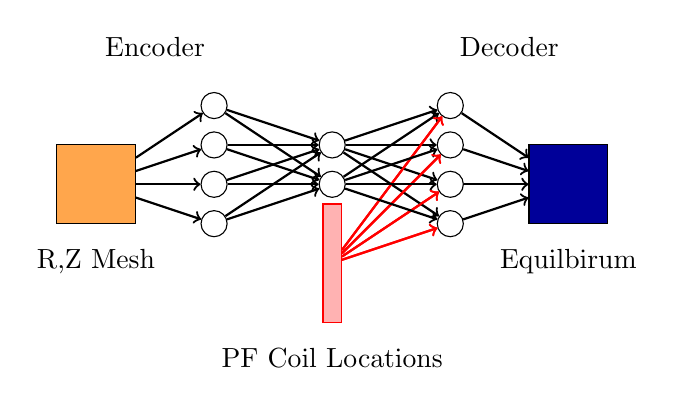
\begin{tikzpicture}[
        scale=0.5, 
        neuron/.style={circle, draw=black, minimum size=0.3cm},
        input image/.style={rectangle, draw=black, minimum width=1cm, minimum height=1cm, fill=orange!70},
        output image/.style={rectangle, draw=black, minimum width=1cm, minimum height=1cm, fill=blue!60!black},
        condition vector/.style={rectangle, draw=red, minimum width=0.2cm, minimum height=1.5cm, fill=red!30},
        arrow/.style={->, thick}
    ]
    
    % Input image
    \node[input image] (input) at (-6,0) {};
    \node[below=0.2cm of input] {R,Z Mesh};
    
    % Encoder layers
    \foreach \x in {1,...,4} {
        \node[neuron] (e\x) at (-3,3-\x) {};
    }
    
    % Latent space
    \foreach \x in {1,...,2} {
        \node[neuron] (l\x) at (0,2-\x) {};
    }
    
    % Conditioning vector
    \node[condition vector] (cond) at (0,-2) {};
    \node[below=0.2cm of cond] {PF Coil Locations};
    
    % Decoder layers
    \foreach \x in {1,...,4} {
        \node[neuron] (d\x) at (3,3-\x) {};
    }
    
    % Output image
    \node[output image] (output) at (6,0) {};
    \node[below=0.2cm of output] {Equilbirum};
    
    % Connections
    % Input to encoder
    \foreach \i in {1,...,4} {
        \draw[arrow] (input) -- (e\i);
    }
    
    % Encoder to latent
    \foreach \i in {1,...,4} {
        \foreach \j in {1,...,2} {
            \draw[arrow] (e\i) -- (l\j);
        }
    }
    
    % Latent and condition to decoder
    \foreach \i in {1,...,2} {
        \foreach \j in {1,...,4} {
            \draw[arrow] (l\i) -- (d\j);
            \draw[arrow, red] (cond) -- (d\j);
        }
    }
    
    % Decoder to output
    \foreach \i in {1,...,4} {
        \draw[arrow] (d\i) -- (output);
    }
    
    % Add labels for components
    \node[align=center] at (-4.5,3.5) {Encoder};
    % \node[align=center] at (0,3.5) {PF Coil\\Locations};
    \node[align=center] at (4.5,3.5) {Decoder};
    
    \end{tikzpicture}
    \caption{Conditional auto-encoder developed as a surrogate model for mapping the poloidal field coil locations to the corresponding magnetic equilibrium under constant coil currents.}
    \label{fig: cae}
\end{figure}



\begin{figure}[h]
    \centering
    \includegraphics[width=\columnwidth]{Images/GS_Pred.pdf}
    \caption{Comparing the ground truth with the prediction from the surrogate model.}
    \label{fig:gs_pred}
\end{figure}



\subsection{Calibration and Validation}
PRE-CP is performed by evaluating the Grad-Shafranov equation over the solution space of the surrogate model, with inputs generated by sampling within the bounds of the PF coil locations. By using the GS equation, we can identify the predictions from the surrogate model that generate untenable equilibria. This allows us to explore the design space quickly while adding trustworthiness to your surrogate model. Both marginal and coverage obtained using PRE-CP with GS equations over the surrogate model is indicated in \cref{fig:gs_coverage}. Marginal-CP shows smooth coverage as it represents the coverage averaged across each cell.


\begin{figure}[h]
    \centering
    \includegraphics[width=0.6\columnwidth]{Images/GS_coverage.pdf}
    \caption{Marginal and joint empirical coverage obtained by performing PRE-CP over the Grad-Shafranov equation}
    \label{fig:gs_coverage}
\end{figure}

\end{document}


